% Options for packages loaded elsewhere
\PassOptionsToPackage{unicode}{hyperref}
\PassOptionsToPackage{hyphens}{url}
%
\documentclass[
  openany]{book}
\usepackage{amsmath,amssymb}
\usepackage{iftex}
\ifPDFTeX
  \usepackage[T1]{fontenc}
  \usepackage[utf8]{inputenc}
  \usepackage{textcomp} % provide euro and other symbols
\else % if luatex or xetex
  \usepackage{unicode-math} % this also loads fontspec
  \defaultfontfeatures{Scale=MatchLowercase}
  \defaultfontfeatures[\rmfamily]{Ligatures=TeX,Scale=1}
\fi
\usepackage{lmodern}
\ifPDFTeX\else
  % xetex/luatex font selection
\fi
% Use upquote if available, for straight quotes in verbatim environments
\IfFileExists{upquote.sty}{\usepackage{upquote}}{}
\IfFileExists{microtype.sty}{% use microtype if available
  \usepackage[]{microtype}
  \UseMicrotypeSet[protrusion]{basicmath} % disable protrusion for tt fonts
}{}
\makeatletter
\@ifundefined{KOMAClassName}{% if non-KOMA class
  \IfFileExists{parskip.sty}{%
    \usepackage{parskip}
  }{% else
    \setlength{\parindent}{0pt}
    \setlength{\parskip}{6pt plus 2pt minus 1pt}}
}{% if KOMA class
  \KOMAoptions{parskip=half}}
\makeatother
\usepackage{xcolor}
\usepackage[margin=3cm]{geometry}
\usepackage{color}
\usepackage{fancyvrb}
\newcommand{\VerbBar}{|}
\newcommand{\VERB}{\Verb[commandchars=\\\{\}]}
\DefineVerbatimEnvironment{Highlighting}{Verbatim}{commandchars=\\\{\}}
% Add ',fontsize=\small' for more characters per line
\usepackage{framed}
\definecolor{shadecolor}{RGB}{248,248,248}
\newenvironment{Shaded}{\begin{snugshade}}{\end{snugshade}}
\newcommand{\AlertTok}[1]{\textcolor[rgb]{0.94,0.16,0.16}{#1}}
\newcommand{\AnnotationTok}[1]{\textcolor[rgb]{0.56,0.35,0.01}{\textbf{\textit{#1}}}}
\newcommand{\AttributeTok}[1]{\textcolor[rgb]{0.13,0.29,0.53}{#1}}
\newcommand{\BaseNTok}[1]{\textcolor[rgb]{0.00,0.00,0.81}{#1}}
\newcommand{\BuiltInTok}[1]{#1}
\newcommand{\CharTok}[1]{\textcolor[rgb]{0.31,0.60,0.02}{#1}}
\newcommand{\CommentTok}[1]{\textcolor[rgb]{0.56,0.35,0.01}{\textit{#1}}}
\newcommand{\CommentVarTok}[1]{\textcolor[rgb]{0.56,0.35,0.01}{\textbf{\textit{#1}}}}
\newcommand{\ConstantTok}[1]{\textcolor[rgb]{0.56,0.35,0.01}{#1}}
\newcommand{\ControlFlowTok}[1]{\textcolor[rgb]{0.13,0.29,0.53}{\textbf{#1}}}
\newcommand{\DataTypeTok}[1]{\textcolor[rgb]{0.13,0.29,0.53}{#1}}
\newcommand{\DecValTok}[1]{\textcolor[rgb]{0.00,0.00,0.81}{#1}}
\newcommand{\DocumentationTok}[1]{\textcolor[rgb]{0.56,0.35,0.01}{\textbf{\textit{#1}}}}
\newcommand{\ErrorTok}[1]{\textcolor[rgb]{0.64,0.00,0.00}{\textbf{#1}}}
\newcommand{\ExtensionTok}[1]{#1}
\newcommand{\FloatTok}[1]{\textcolor[rgb]{0.00,0.00,0.81}{#1}}
\newcommand{\FunctionTok}[1]{\textcolor[rgb]{0.13,0.29,0.53}{\textbf{#1}}}
\newcommand{\ImportTok}[1]{#1}
\newcommand{\InformationTok}[1]{\textcolor[rgb]{0.56,0.35,0.01}{\textbf{\textit{#1}}}}
\newcommand{\KeywordTok}[1]{\textcolor[rgb]{0.13,0.29,0.53}{\textbf{#1}}}
\newcommand{\NormalTok}[1]{#1}
\newcommand{\OperatorTok}[1]{\textcolor[rgb]{0.81,0.36,0.00}{\textbf{#1}}}
\newcommand{\OtherTok}[1]{\textcolor[rgb]{0.56,0.35,0.01}{#1}}
\newcommand{\PreprocessorTok}[1]{\textcolor[rgb]{0.56,0.35,0.01}{\textit{#1}}}
\newcommand{\RegionMarkerTok}[1]{#1}
\newcommand{\SpecialCharTok}[1]{\textcolor[rgb]{0.81,0.36,0.00}{\textbf{#1}}}
\newcommand{\SpecialStringTok}[1]{\textcolor[rgb]{0.31,0.60,0.02}{#1}}
\newcommand{\StringTok}[1]{\textcolor[rgb]{0.31,0.60,0.02}{#1}}
\newcommand{\VariableTok}[1]{\textcolor[rgb]{0.00,0.00,0.00}{#1}}
\newcommand{\VerbatimStringTok}[1]{\textcolor[rgb]{0.31,0.60,0.02}{#1}}
\newcommand{\WarningTok}[1]{\textcolor[rgb]{0.56,0.35,0.01}{\textbf{\textit{#1}}}}
\usepackage{longtable,booktabs,array}
\usepackage{calc} % for calculating minipage widths
% Correct order of tables after \paragraph or \subparagraph
\usepackage{etoolbox}
\makeatletter
\patchcmd\longtable{\par}{\if@noskipsec\mbox{}\fi\par}{}{}
\makeatother
% Allow footnotes in longtable head/foot
\IfFileExists{footnotehyper.sty}{\usepackage{footnotehyper}}{\usepackage{footnote}}
\makesavenoteenv{longtable}
\usepackage{graphicx}
\makeatletter
\def\maxwidth{\ifdim\Gin@nat@width>\linewidth\linewidth\else\Gin@nat@width\fi}
\def\maxheight{\ifdim\Gin@nat@height>\textheight\textheight\else\Gin@nat@height\fi}
\makeatother
% Scale images if necessary, so that they will not overflow the page
% margins by default, and it is still possible to overwrite the defaults
% using explicit options in \includegraphics[width, height, ...]{}
\setkeys{Gin}{width=\maxwidth,height=\maxheight,keepaspectratio}
% Set default figure placement to htbp
\makeatletter
\def\fps@figure{htbp}
\makeatother
\setlength{\emergencystretch}{3em} % prevent overfull lines
\providecommand{\tightlist}{%
  \setlength{\itemsep}{0pt}\setlength{\parskip}{0pt}}
\setcounter{secnumdepth}{5}
\usepackage{booktabs}
\ifLuaTeX
  \usepackage{selnolig}  % disable illegal ligatures
\fi
\usepackage[]{natbib}
\bibliographystyle{plainnat}
\usepackage{bookmark}
\IfFileExists{xurl.sty}{\usepackage{xurl}}{} % add URL line breaks if available
\urlstyle{same}
\hypersetup{
  pdftitle={Linear Methods for Data Science Notes},
  pdfauthor={John Michael Epperson},
  hidelinks,
  pdfcreator={LaTeX via pandoc}}

\title{Linear Methods for Data Science Notes}
\author{John Michael Epperson}
\date{}

\begin{document}
\maketitle

{
\setcounter{tocdepth}{1}
\tableofcontents
}
\chapter*{About}\label{about}
\addcontentsline{toc}{chapter}{About}

These are my notes for the Fall 2024 session of STAT 6021: Linear Methods for Data Science at the School of Data Science at the University of Virginia.

The course is taught by Jeffrey Woo.

\chapter*{Syllabus Week}\label{syllabus-week}
\addcontentsline{toc}{chapter}{Syllabus Week}

\section{Agenda}\label{agenda}

\begin{itemize}
\tightlist
\item
  Welcome
\item
  Live Session
\item
  Some logistical tips
\item
  Meet group members
\item
  Q\&A on Protocol and Policies
\item
  Q\&A on Modules A \& B (Review Material)
\end{itemize}

\chapter{Data Wrangling with R}\label{data-wrangling-with-r}

\section*{Cheat Sheet}\label{cheat-sheet}
\addcontentsline{toc}{section}{Cheat Sheet}

\begin{itemize}
\tightlist
\item
  pipes ``\%\textgreater\%'' are interpreted as `and then' in code

  \begin{itemize}
  \tightlist
  \item
    can be typed or accessed by Ctrl+Alt+M
  \end{itemize}
\end{itemize}

\section{Data Wrangling Using Base R Functions}\label{data-wrangling-using-base-r-functions}

\begin{Shaded}
\begin{Highlighting}[]
\NormalTok{Data}\OtherTok{\textless{}{-}}\FunctionTok{read.csv}\NormalTok{(}\StringTok{"datasets/ClassDataPrevious.csv"}\NormalTok{,}\AttributeTok{header =} \ConstantTok{TRUE}\NormalTok{)}
\FunctionTok{dim}\NormalTok{(Data)}
\end{Highlighting}
\end{Shaded}

\begin{verbatim}
## [1] 298   8
\end{verbatim}

\begin{Shaded}
\begin{Highlighting}[]
\FunctionTok{colnames}\NormalTok{(Data)}
\end{Highlighting}
\end{Shaded}

\begin{verbatim}
## [1] "Year"     "Sleep"    "Sport"    "Courses"  "Major"    "Age"      "Computer"
## [8] "Lunch"
\end{verbatim}

\begin{Shaded}
\begin{Highlighting}[]
\NormalTok{Data[}\DecValTok{1}\NormalTok{,}\DecValTok{2}\NormalTok{]}
\end{Highlighting}
\end{Shaded}

\begin{verbatim}
## [1] 8
\end{verbatim}

\begin{Shaded}
\begin{Highlighting}[]
\NormalTok{Data[}\FunctionTok{c}\NormalTok{(}\DecValTok{1}\NormalTok{,}\DecValTok{3}\NormalTok{,}\DecValTok{4}\NormalTok{),}\FunctionTok{c}\NormalTok{(}\DecValTok{1}\NormalTok{,}\DecValTok{5}\NormalTok{,}\DecValTok{8}\NormalTok{)]}
\end{Highlighting}
\end{Shaded}

\begin{verbatim}
##     Year                            Major Lunch
## 1 Second                         Commerce    11
## 3 Second Cognitive science and psychology    10
## 4  First                         Pre-Comm     4
\end{verbatim}

To view a column

\begin{Shaded}
\begin{Highlighting}[]
\NormalTok{Data}\SpecialCharTok{$}\NormalTok{Year}
\NormalTok{Data[,}\DecValTok{1}\NormalTok{]}
\NormalTok{Data[,}\SpecialCharTok{{-}}\FunctionTok{c}\NormalTok{(}\DecValTok{2}\SpecialCharTok{:}\DecValTok{8}\NormalTok{)]}
\end{Highlighting}
\end{Shaded}

\begin{Shaded}
\begin{Highlighting}[]
\FunctionTok{which}\NormalTok{(Data}\SpecialCharTok{$}\NormalTok{Sport}\SpecialCharTok{==}\StringTok{"Soccer"}\NormalTok{)}
\end{Highlighting}
\end{Shaded}

\begin{verbatim}
##  [1]   3  20  25  26  31  32  33  38  44  46  48  50  51  64  67  71  87  92  98
## [20]  99 118 122 124 126 128 133 136 137 143 146 153 159 165 174 197 198 207 211
## [39] 214 226 234 241 255 259 260 266 274 278 281 283 294 295
\end{verbatim}

\begin{Shaded}
\begin{Highlighting}[]
\NormalTok{SoccerPeeps}\OtherTok{\textless{}{-}}\NormalTok{Data[}\FunctionTok{which}\NormalTok{(Data}\SpecialCharTok{$}\NormalTok{Sport}\SpecialCharTok{==}\StringTok{"Soccer"}\NormalTok{),]}
\FunctionTok{dim}\NormalTok{(SoccerPeeps)}
\end{Highlighting}
\end{Shaded}

\begin{verbatim}
## [1] 52  8
\end{verbatim}

\begin{Shaded}
\begin{Highlighting}[]
\NormalTok{SoccerPeeps\_2nd}\OtherTok{\textless{}{-}}\NormalTok{Data[}\FunctionTok{which}\NormalTok{(Data}\SpecialCharTok{$}\NormalTok{Sport}\SpecialCharTok{==}\StringTok{"Soccer"} \SpecialCharTok{\&}\NormalTok{ Data}\SpecialCharTok{$}\NormalTok{Year}\SpecialCharTok{==}\StringTok{"Second"}\NormalTok{),]}
\FunctionTok{dim}\NormalTok{(SoccerPeeps\_2nd)}
\end{Highlighting}
\end{Shaded}

\begin{verbatim}
## [1] 25  8
\end{verbatim}

\begin{Shaded}
\begin{Highlighting}[]
\NormalTok{Sleepy}\OtherTok{\textless{}{-}}\NormalTok{Data[}\FunctionTok{which}\NormalTok{(Data}\SpecialCharTok{$}\NormalTok{Sleep}\SpecialCharTok{\textgreater{}}\DecValTok{8}\NormalTok{),]}
\end{Highlighting}
\end{Shaded}

\subsection{Changing Column Names}\label{changing-column-names}

\begin{Shaded}
\begin{Highlighting}[]
\FunctionTok{names}\NormalTok{(Data)[}\FunctionTok{c}\NormalTok{(}\DecValTok{1}\NormalTok{,}\DecValTok{7}\NormalTok{)]}\OtherTok{\textless{}{-}}\FunctionTok{c}\NormalTok{(}\StringTok{"Yr"}\NormalTok{,}\StringTok{"Computer"}\NormalTok{)}
\end{Highlighting}
\end{Shaded}

Find and remove missing data

\begin{Shaded}
\begin{Highlighting}[]
\FunctionTok{is.na}\NormalTok{(Data)}
\end{Highlighting}
\end{Shaded}

\begin{Shaded}
\begin{Highlighting}[]
\NormalTok{Data[}\SpecialCharTok{!}\FunctionTok{complete.cases}\NormalTok{(Data),]}
\end{Highlighting}
\end{Shaded}

\begin{verbatim}
##         Yr Sleep      Sport Courses                                      Major
## 103 Second    NA Basketball       7 psychology and youth and social innovation
## 206 Second     8       None       4                          Cognitive Science
##     Age Computer Lunch
## 103  19      Mac    10
## 206  19      Mac    NA
\end{verbatim}

\subsection{\texorpdfstring{\textbf{Summarizing Variables}}{Summarizing Variables}}\label{summarizing-variables}

\begin{Shaded}
\begin{Highlighting}[]
\FunctionTok{apply}\NormalTok{(Data[,}\FunctionTok{c}\NormalTok{(}\DecValTok{2}\NormalTok{,}\DecValTok{4}\NormalTok{,}\DecValTok{6}\NormalTok{,}\DecValTok{8}\NormalTok{)],}\DecValTok{2}\NormalTok{,mean)}
\end{Highlighting}
\end{Shaded}

\begin{verbatim}
##     Sleep   Courses       Age     Lunch 
##        NA  5.016779 19.573826        NA
\end{verbatim}

To not include missing values, use arg na.rm

\begin{Shaded}
\begin{Highlighting}[]
\FunctionTok{apply}\NormalTok{(Data[,}\FunctionTok{c}\NormalTok{(}\DecValTok{2}\NormalTok{,}\DecValTok{4}\NormalTok{,}\DecValTok{6}\NormalTok{,}\DecValTok{8}\NormalTok{)],}\DecValTok{2}\NormalTok{,mean,}\AttributeTok{na.rm=}\NormalTok{T)}
\end{Highlighting}
\end{Shaded}

\begin{verbatim}
##      Sleep    Courses        Age      Lunch 
## 155.559259   5.016779  19.573826 156.594175
\end{verbatim}

In apply(), the second argument specifies whether to summarize row (put 1) or column (put 2) values

Since some of the means are very high, we can use the median instead to be a little more informative.

\begin{Shaded}
\begin{Highlighting}[]
\FunctionTok{apply}\NormalTok{(Data[,}\FunctionTok{c}\NormalTok{(}\DecValTok{2}\NormalTok{,}\DecValTok{4}\NormalTok{,}\DecValTok{6}\NormalTok{,}\DecValTok{8}\NormalTok{)],}\DecValTok{2}\NormalTok{,median,}\AttributeTok{na.rm=}\NormalTok{T)}
\end{Highlighting}
\end{Shaded}

\begin{verbatim}
##   Sleep Courses     Age   Lunch 
##     7.5     5.0    19.0     9.0
\end{verbatim}

\subsection{\texorpdfstring{\textbf{Summarizing variable by groups}}{Summarizing variable by groups}}\label{summarizing-variable-by-groups}

use tapply()

\begin{Shaded}
\begin{Highlighting}[]
\FunctionTok{tapply}\NormalTok{(Data}\SpecialCharTok{$}\NormalTok{Sleep,Data}\SpecialCharTok{$}\NormalTok{Yr,median,}\AttributeTok{na.rm=}\NormalTok{T)}
\end{Highlighting}
\end{Shaded}

\begin{verbatim}
##  First Fourth Second  Third 
##    8.0    7.0    7.5    7.0
\end{verbatim}

\begin{Shaded}
\begin{Highlighting}[]
\NormalTok{Data}\SpecialCharTok{$}\NormalTok{Yr}\OtherTok{\textless{}{-}}\FunctionTok{factor}\NormalTok{(Data}\SpecialCharTok{$}\NormalTok{Yr,}\AttributeTok{levels=}\FunctionTok{c}\NormalTok{(}\StringTok{"First"}\NormalTok{,}\StringTok{"Second"}\NormalTok{,}\StringTok{"Third"}\NormalTok{,}\StringTok{"Fourth"}\NormalTok{))}
\FunctionTok{levels}\NormalTok{(Data}\SpecialCharTok{$}\NormalTok{Yr)}
\end{Highlighting}
\end{Shaded}

\begin{verbatim}
## [1] "First"  "Second" "Third"  "Fourth"
\end{verbatim}

\begin{Shaded}
\begin{Highlighting}[]
\FunctionTok{tapply}\NormalTok{(Data}\SpecialCharTok{$}\NormalTok{Sleep,Data}\SpecialCharTok{$}\NormalTok{Yr,median,}\AttributeTok{na.rm=}\NormalTok{T)}
\end{Highlighting}
\end{Shaded}

\begin{verbatim}
##  First Second  Third Fourth 
##    8.0    7.5    7.0    7.0
\end{verbatim}

\begin{Shaded}
\begin{Highlighting}[]
\FunctionTok{tapply}\NormalTok{(Data}\SpecialCharTok{$}\NormalTok{Sleep,}\FunctionTok{list}\NormalTok{(Data}\SpecialCharTok{$}\NormalTok{Yr,Data}\SpecialCharTok{$}\NormalTok{Computer),median,}\AttributeTok{na.rm=}\NormalTok{T)}
\end{Highlighting}
\end{Shaded}

\begin{verbatim}
##           Mac   PC
## First  NA 8.0 7.50
## Second  7 7.5 7.50
## Third  NA 7.5 7.00
## Fourth NA 7.0 7.25
\end{verbatim}

\subsection{\texorpdfstring{\textbf{Create a new variable based on existing variable}}{Create a new variable based on existing variable}}\label{create-a-new-variable-based-on-existing-variable}

\begin{Shaded}
\begin{Highlighting}[]
\NormalTok{sleep\_mins}\OtherTok{\textless{}{-}}\NormalTok{Data}\SpecialCharTok{$}\NormalTok{Sleep}\SpecialCharTok{*}\DecValTok{60}
\NormalTok{deprived}\OtherTok{\textless{}{-}}\FunctionTok{ifelse}\NormalTok{(Data}\SpecialCharTok{$}\NormalTok{Sleep}\SpecialCharTok{\textless{}}\DecValTok{7}\NormalTok{,}\StringTok{"yes"}\NormalTok{,}\StringTok{"no"}\NormalTok{)}
\end{Highlighting}
\end{Shaded}

Create catagorical variable based on numerical value

\begin{Shaded}
\begin{Highlighting}[]
\NormalTok{CourseLoad}\OtherTok{\textless{}{-}}\FunctionTok{cut}\NormalTok{(Data}\SpecialCharTok{$}\NormalTok{Courses,}\AttributeTok{breaks=}\FunctionTok{c}\NormalTok{(}\SpecialCharTok{{-}}\ConstantTok{Inf}\NormalTok{,}\DecValTok{3}\NormalTok{,}\DecValTok{5}\NormalTok{,}\ConstantTok{Inf}\NormalTok{),}\AttributeTok{labels=}\FunctionTok{c}\NormalTok{(}\StringTok{"light"}\NormalTok{,}\StringTok{"regular"}\NormalTok{,}\StringTok{"heavy"}\NormalTok{))}
\end{Highlighting}
\end{Shaded}

Collapse levels
into upperclassmen and lowerclassmen

\begin{Shaded}
\begin{Highlighting}[]
\FunctionTok{levels}\NormalTok{(Data}\SpecialCharTok{$}\NormalTok{Yr)}
\end{Highlighting}
\end{Shaded}

\begin{verbatim}
## [1] "First"  "Second" "Third"  "Fourth"
\end{verbatim}

\begin{Shaded}
\begin{Highlighting}[]
\NormalTok{new.levels}\OtherTok{\textless{}{-}}\FunctionTok{c}\NormalTok{(}\StringTok{"und"}\NormalTok{,}\StringTok{"und"}\NormalTok{,}\StringTok{"up"}\NormalTok{,}\StringTok{"up"}\NormalTok{)}
\NormalTok{Year2}\OtherTok{\textless{}{-}}\FunctionTok{factor}\NormalTok{(new.levels[Data}\SpecialCharTok{$}\NormalTok{Yr])}
\FunctionTok{levels}\NormalTok{(Year2)}
\end{Highlighting}
\end{Shaded}

\begin{verbatim}
## [1] "und" "up"
\end{verbatim}

\subsection{\texorpdfstring{\textbf{Combine data frames}}{Combine data frames}}\label{combine-data-frames}

\begin{Shaded}
\begin{Highlighting}[]
\NormalTok{Data}\OtherTok{\textless{}{-}}\FunctionTok{data.frame}\NormalTok{(Data,sleep\_mins,deprived,CourseLoad,Year2)}
\FunctionTok{head}\NormalTok{(Data)}
\end{Highlighting}
\end{Shaded}

\begin{verbatim}
##       Yr Sleep      Sport Courses                            Major Age Computer
## 1 Second     8 Basketball       6                         Commerce  19      Mac
## 2 Second     7     Tennis       5                       Psychology  19      Mac
## 3 Second     8     Soccer       5 Cognitive science and psychology  21      Mac
## 4  First     9 Basketball       5                         Pre-Comm  19      Mac
## 5 Second     4 Basketball       6                      Statistics   19       PC
## 6  Third     7       None       4                       Psychology  20       PC
##   Lunch sleep_mins deprived CourseLoad Year2
## 1    11        480       no      heavy   und
## 2    10        420       no    regular   und
## 3    10        480       no    regular   und
## 4     4        540       no    regular   und
## 5     0        240      yes      heavy   und
## 6    11        420       no    regular    up
\end{verbatim}

Can use cbind() alternatively for same result

\begin{Shaded}
\begin{Highlighting}[]
\NormalTok{Data2}\OtherTok{\textless{}{-}}\FunctionTok{cbind}\NormalTok{(Data,sleep\_mins,deprived,CourseLoad,Year2)}
\end{Highlighting}
\end{Shaded}

When combining data frames which have different observations but the same columns, we can merge them using rbind()

\begin{Shaded}
\begin{Highlighting}[]
\NormalTok{dat1}\OtherTok{\textless{}{-}}\NormalTok{Data[}\DecValTok{1}\SpecialCharTok{:}\DecValTok{3}\NormalTok{,}\DecValTok{1}\SpecialCharTok{:}\DecValTok{3}\NormalTok{]}
\NormalTok{dat3}\OtherTok{\textless{}{-}}\NormalTok{Data[}\DecValTok{6}\SpecialCharTok{:}\DecValTok{8}\NormalTok{,}\DecValTok{1}\SpecialCharTok{:}\DecValTok{3}\NormalTok{]}
\NormalTok{res.dat2}\OtherTok{\textless{}{-}}\FunctionTok{rbind}\NormalTok{(dat1,dat3)}
\FunctionTok{head}\NormalTok{(res.dat2)}
\end{Highlighting}
\end{Shaded}

\begin{verbatim}
##       Yr Sleep      Sport
## 1 Second     8 Basketball
## 2 Second     7     Tennis
## 3 Second     8     Soccer
## 6  Third     7       None
## 7 Second     7 Basketball
## 8  First     7 Basketball
\end{verbatim}

**Export data frame to csv

\begin{Shaded}
\begin{Highlighting}[]
\FunctionTok{write.csv}\NormalTok{(Data,}\AttributeTok{file=}\StringTok{"exports/newdata.csv"}\NormalTok{,}\AttributeTok{row.names=}\ConstantTok{FALSE}\NormalTok{)}
\end{Highlighting}
\end{Shaded}

\subsection{\texorpdfstring{\textbf{Sort data frame by column values}}{Sort data frame by column values}}\label{sort-data-frame-by-column-values}

to sort in ascending order by age, then descending

\begin{Shaded}
\begin{Highlighting}[]
\NormalTok{Data\_by\_age}\OtherTok{\textless{}{-}}\NormalTok{Data[}\FunctionTok{order}\NormalTok{(Data}\SpecialCharTok{$}\NormalTok{Age),]}
\NormalTok{Data\_by\_age\_des}\OtherTok{\textless{}{-}}\NormalTok{Data[}\FunctionTok{order}\NormalTok{(}\SpecialCharTok{{-}}\NormalTok{Data}\SpecialCharTok{$}\NormalTok{Age),]}
\end{Highlighting}
\end{Shaded}

To sort ascending by age then by sleep:

\begin{Shaded}
\begin{Highlighting}[]
\NormalTok{Data\_by\_age\_sleep}\OtherTok{\textless{}{-}}\NormalTok{Data[}\FunctionTok{order}\NormalTok{(Data}\SpecialCharTok{$}\NormalTok{Age, Data}\SpecialCharTok{$}\NormalTok{Sleep),]}
\end{Highlighting}
\end{Shaded}

\begin{center}\rule{0.5\linewidth}{0.5pt}\end{center}

\section{Data Wrangling Using dplyr Functions}\label{data-wrangling-using-dplyr-functions}

First we'll clear our environment using rm(list=ls()), then load tidyverse, which contains the dplyr functions:

\begin{Shaded}
\begin{Highlighting}[]
\FunctionTok{rm}\NormalTok{(}\AttributeTok{list=}\FunctionTok{ls}\NormalTok{())}
\FunctionTok{library}\NormalTok{(tidyverse)}
\end{Highlighting}
\end{Shaded}

\begin{verbatim}
## -- Attaching core tidyverse packages ----------------- tidyverse 2.0.0 --
## v dplyr     1.1.4     v readr     2.1.5
## v forcats   1.0.0     v stringr   1.5.1
## v ggplot2   3.5.1     v tibble    3.2.1
## v lubridate 1.9.3     v tidyr     1.3.1
## v purrr     1.0.2     
## -- Conflicts ----------------------------------- tidyverse_conflicts() --
## x dplyr::filter() masks stats::filter()
## x dplyr::lag()    masks stats::lag()
## i Use the conflicted package (<http://conflicted.r-lib.org/>) to force all conflicts to become errors
\end{verbatim}

\begin{Shaded}
\begin{Highlighting}[]
\NormalTok{Data}\OtherTok{\textless{}{-}}\FunctionTok{read.csv}\NormalTok{(}\StringTok{"datasets/ClassDataPrevious.csv"}\NormalTok{,}\AttributeTok{header=}\ConstantTok{TRUE}\NormalTok{)}
\end{Highlighting}
\end{Shaded}

\subsection{Select Specific Columns of a Data Fram}\label{select-specific-columns-of-a-data-fram}

use select() function, two ways to do it

Or use \textbf{Pipes}

Pipes can be typed using either \%\textgreater\% or Ctrl+Shift+M on keyboard. To thing of the operations above, we can read the code as:

\begin{enumerate}
\def\labelenumi{\arabic{enumi}.}
\tightlist
\item
  Take the data frame called Data
\item
  and then select the column named Year
\end{enumerate}

In this way, we can interpret a pipe as ``and then''. Commands after pipe should be placed on a new line. Pipes are especially useful for lots of sequential commands.

\subsection{Select observations by conditions}\label{select-observations-by-conditions}

The \textbf{filter()} function allows us to subset our data based on some conditions, for example, to select students whose favorite sport is soccer:

or use a pipe to store results in a new variable ``SoccerPeeps''

\begin{Shaded}
\begin{Highlighting}[]
\NormalTok{SoccerPeeps}\OtherTok{\textless{}{-}}\NormalTok{Data }\SpecialCharTok{\%\textgreater{}\%} 
  \FunctionTok{filter}\NormalTok{(Sport}\SpecialCharTok{==}\StringTok{"Soccer"}\NormalTok{)}

\NormalTok{SoccerPeeps\_2nd}\OtherTok{\textless{}{-}}\NormalTok{Data }\SpecialCharTok{\%\textgreater{}\%} 
  \FunctionTok{filter}\NormalTok{(Sport}\SpecialCharTok{==}\StringTok{"Soccer"} \SpecialCharTok{\&}\NormalTok{ Year}\SpecialCharTok{==}\StringTok{"Second"}\NormalTok{)}

\NormalTok{Sleepy}\OtherTok{\textless{}{-}}\NormalTok{Data }\SpecialCharTok{\%\textgreater{}\%} 
  \FunctionTok{filter}\NormalTok{(Sleep}\SpecialCharTok{\textgreater{}}\DecValTok{8}\NormalTok{)}

\NormalTok{Sleepy\_or\_Soccer}\OtherTok{\textless{}{-}}\NormalTok{Data }\SpecialCharTok{\%\textgreater{}\%} 
  \FunctionTok{filter}\NormalTok{(Sport}\SpecialCharTok{==}\StringTok{"Soccer"}\SpecialCharTok{|}\NormalTok{Sleep}\SpecialCharTok{\textgreater{}}\DecValTok{8}\NormalTok{)}
\end{Highlighting}
\end{Shaded}

\subsection{Change Column Name}\label{change-column-name}

Changing the names of columns is easy with dplyr, use rename() function

\begin{Shaded}
\begin{Highlighting}[]
\NormalTok{Data}\OtherTok{\textless{}{-}}\NormalTok{Data }\SpecialCharTok{\%\textgreater{}\%} 
  \FunctionTok{rename}\NormalTok{(}\AttributeTok{Yr=}\NormalTok{Year,}\AttributeTok{Comp=}\NormalTok{Computer)}
\end{Highlighting}
\end{Shaded}

\subsection{Summarizing Variables}\label{summarizing-variables-1}

The summarize() function allows us to summarize a column. Suppose we want to find the mean value of the numeric columns: Sleep, Courses, Age, Lunch:

\begin{Shaded}
\begin{Highlighting}[]
\NormalTok{Data }\SpecialCharTok{\%\textgreater{}\%} 
  \FunctionTok{summarize}\NormalTok{(}\FunctionTok{mean}\NormalTok{(Sleep,}\AttributeTok{na.rm=}\NormalTok{T),}\FunctionTok{mean}\NormalTok{(Courses),}\FunctionTok{mean}\NormalTok{(Age),}\FunctionTok{mean}\NormalTok{(Lunch,}\AttributeTok{na.rm=}\NormalTok{T))}
\end{Highlighting}
\end{Shaded}

\begin{verbatim}
##   mean(Sleep, na.rm = T) mean(Courses) mean(Age) mean(Lunch, na.rm = T)
## 1               155.5593      5.016779  19.57383               156.5942
\end{verbatim}

This output is cumbersome, but we can give names to each summary:

\begin{Shaded}
\begin{Highlighting}[]
\NormalTok{Data }\SpecialCharTok{\%\textgreater{}\%} 
  \FunctionTok{summarize}\NormalTok{(}\AttributeTok{avgSleep=}\FunctionTok{mean}\NormalTok{(Sleep,}\AttributeTok{na.rm =}\NormalTok{ T),}\AttributeTok{avgCourse=}\FunctionTok{mean}\NormalTok{(Courses,}\AttributeTok{na.rm =}\NormalTok{ T),}\AttributeTok{avgAge=}\FunctionTok{mean}\NormalTok{(Age,}\AttributeTok{na.rm=}\NormalTok{T),}\AttributeTok{avgLun=}\FunctionTok{mean}\NormalTok{(Lunch,}\AttributeTok{na.rm =}\NormalTok{ T))}
\end{Highlighting}
\end{Shaded}

\begin{verbatim}
##   avgSleep avgCourse   avgAge   avgLun
## 1 155.5593  5.016779 19.57383 156.5942
\end{verbatim}

As previously seen, some of these variables are suspiciously high, we can use the median instead of mean to get more informative results:

\begin{Shaded}
\begin{Highlighting}[]
\NormalTok{Data }\SpecialCharTok{\%\textgreater{}\%} 
  \FunctionTok{summarize}\NormalTok{(}\AttributeTok{avgSleep=}\FunctionTok{median}\NormalTok{(Sleep,}\AttributeTok{na.rm =}\NormalTok{ T),}\AttributeTok{avgCourse=}\FunctionTok{median}\NormalTok{(Courses,}\AttributeTok{na.rm =}\NormalTok{ T),}\AttributeTok{avgAge=}\FunctionTok{median}\NormalTok{(Age,}\AttributeTok{na.rm=}\NormalTok{T),}\AttributeTok{avgLun=}\FunctionTok{median}\NormalTok{(Lunch,}\AttributeTok{na.rm =}\NormalTok{ T))}
\end{Highlighting}
\end{Shaded}

\begin{verbatim}
##   avgSleep avgCourse avgAge avgLun
## 1      7.5         5     19      9
\end{verbatim}

\subsection{Summarizing Variable by Groups}\label{summarizing-variable-by-groups-1}

If we want to find the median amount of sleep for 1st, 2nd, 3rd, and 4th years, we can use the `group\_by()' function.

\begin{Shaded}
\begin{Highlighting}[]
\NormalTok{Data }\SpecialCharTok{\%\textgreater{}\%} 
  \FunctionTok{group\_by}\NormalTok{(Yr) }\SpecialCharTok{\%\textgreater{}\%} 
  \FunctionTok{summarize}\NormalTok{(}\AttributeTok{medSleep=}\FunctionTok{median}\NormalTok{(Sleep,}\AttributeTok{na.rm=}\NormalTok{T))}
\end{Highlighting}
\end{Shaded}

\begin{verbatim}
## # A tibble: 4 x 2
##   Yr     medSleep
##   <chr>     <dbl>
## 1 First       8  
## 2 Fourth      7  
## 3 Second      7.5
## 4 Third       7
\end{verbatim}

The way we can read the code is:
1. Get the data frame called Data,
2. and then group the observations by Yr,
3. and the find the median amount of sleep by each Yr and store the median in a vector called medSleep

The order of the factor levels is in alphabetical, which isn't very useful. We can use the `mutate()' function whenever we want to transform or create a new variable. In this case, we are transforming the variable `Yr' by reordering the factor levels with the `fct\_relevel()' function:

\begin{Shaded}
\begin{Highlighting}[]
\NormalTok{Data}\OtherTok{\textless{}{-}}\NormalTok{Data }\SpecialCharTok{\%\textgreater{}\%} 
  \FunctionTok{mutate}\NormalTok{(Yr}\OtherTok{\textless{}{-}}\NormalTok{Yr }\SpecialCharTok{\%\textgreater{}\%} 
           \FunctionTok{fct\_relevel}\NormalTok{(}\FunctionTok{c}\NormalTok{(}\StringTok{"First"}\NormalTok{,}\StringTok{"Second"}\NormalTok{,}\StringTok{"Third"}\NormalTok{,}\StringTok{"Fourth"}\NormalTok{)))}
\end{Highlighting}
\end{Shaded}

which reads:
1. Get data frame called `Data',
2. and then transform the variable called `Yr',
3. and then reorder the factor levels

then we use pipes, the `group\_by()', and `summarize()' functions like before:

\begin{Shaded}
\begin{Highlighting}[]
\NormalTok{Data }\SpecialCharTok{\%\textgreater{}\%} 
  \FunctionTok{group\_by}\NormalTok{(Yr) }\SpecialCharTok{\%\textgreater{}\%} 
  \FunctionTok{summarize}\NormalTok{(}\AttributeTok{medSleep=}\FunctionTok{median}\NormalTok{(Sleep,}\AttributeTok{na.rm=}\NormalTok{T))}
\end{Highlighting}
\end{Shaded}

\begin{verbatim}
## # A tibble: 4 x 2
##   Yr     medSleep
##   <chr>     <dbl>
## 1 First       8  
## 2 Fourth      7  
## 3 Second      7.5
## 4 Third       7
\end{verbatim}

This output makes a lot more sense for this context.

To summarize a variable on groups formed by more than one variable, we just add the other variables in the `group\_by()' function:

\begin{Shaded}
\begin{Highlighting}[]
\NormalTok{Data }\SpecialCharTok{\%\textgreater{}\%} 
  \FunctionTok{group\_by}\NormalTok{(Yr,Comp) }\SpecialCharTok{\%\textgreater{}\%} 
  \FunctionTok{summarize}\NormalTok{(}\AttributeTok{medSleep=}\FunctionTok{median}\NormalTok{(Sleep,}\AttributeTok{na.rm=}\NormalTok{T))}
\end{Highlighting}
\end{Shaded}

\begin{verbatim}
## `summarise()` has grouped output by 'Yr'. You can override using the
## `.groups` argument.
\end{verbatim}

\begin{verbatim}
## # A tibble: 9 x 3
## # Groups:   Yr [4]
##   Yr     Comp  medSleep
##   <chr>  <chr>    <dbl>
## 1 First  "Mac"     8   
## 2 First  "PC"      7.5 
## 3 Fourth "Mac"     7   
## 4 Fourth "PC"      7.25
## 5 Second ""        7   
## 6 Second "Mac"     7.5 
## 7 Second "PC"      7.5 
## 8 Third  "Mac"     7.5 
## 9 Third  "PC"      7
\end{verbatim}

\subsection{Create a New Variable Based on Existing Variable(s)}\label{create-a-new-variable-based-on-existing-variables}

As mentioned previously, the `mutate()' function is used to transform a variable or to create a new variable. There are a few variations on this task, based on the type of variable you want to create, and the type of variable it is based on.

\textbf{Create a numeric variable based on another numerica variable}

The variable `Sleep' is in number of hours. Suppose we need to convert the values of `Sleep' to number of minutes, we can simply perform the following mathematical operation:

\begin{Shaded}
\begin{Highlighting}[]
\NormalTok{Data}\OtherTok{\textless{}{-}}\NormalTok{Data }\SpecialCharTok{\%\textgreater{}\%} 
  \FunctionTok{mutate}\NormalTok{(}\AttributeTok{Sleep\_mins=}\NormalTok{Sleep}\SpecialCharTok{*}\DecValTok{60}\NormalTok{)}
\end{Highlighting}
\end{Shaded}

and store the transformed variable called `Sleep\_mins' and add `Sleep\_mins' to the data frame called `Data'.

\textbf{Create a binary variable based on a numeric variable}

Create binary variable called `deprived'. An observation will obtain a value of `yes' if they sleep less than 7 hours a night, and `no' otherwise. We will then add this variable to the data frame called `Data':

\begin{Shaded}
\begin{Highlighting}[]
\NormalTok{Data}\OtherTok{\textless{}{-}}\NormalTok{Data }\SpecialCharTok{\%\textgreater{}\%} 
  \FunctionTok{mutate}\NormalTok{(}\AttributeTok{deprived=}\FunctionTok{ifelse}\NormalTok{(Sleep}\SpecialCharTok{\textless{}}\DecValTok{7}\NormalTok{,}\StringTok{"yes"}\NormalTok{,}\StringTok{"no"}\NormalTok{))}
\end{Highlighting}
\end{Shaded}

\textbf{Create a categorical variable based on a numeric variable}

Suppose we want to create a categorical variable based on the number of courses a student takes. We will call this new variable `CourseLoad', which takes on the following variables

\begin{itemize}
\tightlist
\item
  `light' if 3 courses or less
\item
  `regular' if 4 or 5 courses
\item
  `heavy' if more than 5 courses
\end{itemize}

and then add `CourseLoad to the data frame 'Data'. We can use the `case\_when()' function from the `dplyr' package, instead of the `cut()' function:

\begin{Shaded}
\begin{Highlighting}[]
\NormalTok{Data}\OtherTok{\textless{}{-}}\NormalTok{Data }\SpecialCharTok{\%\textgreater{}\%} 
  \FunctionTok{mutate}\NormalTok{(}\AttributeTok{CourseLoad=}\FunctionTok{case\_when}\NormalTok{(Courses}\SpecialCharTok{\textless{}=}\DecValTok{3} \SpecialCharTok{\textasciitilde{}} \StringTok{"light"}\NormalTok{,}
\NormalTok{                              Courses}\SpecialCharTok{\textgreater{}}\DecValTok{3} \SpecialCharTok{\&}\NormalTok{ Courses }\SpecialCharTok{\textless{}=}\DecValTok{5} \SpecialCharTok{\textasciitilde{}}\StringTok{"regular"}\NormalTok{,}
\NormalTok{                              Courses}\SpecialCharTok{\textgreater{}}\DecValTok{5} \SpecialCharTok{\textasciitilde{}} \StringTok{"heavy"}\NormalTok{))}
\end{Highlighting}
\end{Shaded}

Note how the category names are suppied after a specific condition is specified.

\textbf{Collapsing Levels}

Sometimes a categorical variable has more levels than needed, so we may want to collapse the levels, as such in this case: collapsing `Year' into upperclassmen and lowerclassmen.

\begin{Shaded}
\begin{Highlighting}[]
\NormalTok{Data}\OtherTok{\textless{}{-}}\NormalTok{Data }\SpecialCharTok{\%\textgreater{}\%} 
  \FunctionTok{mutate}\NormalTok{(}\AttributeTok{UpUnder=}\FunctionTok{fct\_collapse}\NormalTok{(Yr,}\AttributeTok{under=}\FunctionTok{c}\NormalTok{(}\StringTok{"First"}\NormalTok{,}\StringTok{"Second"}\NormalTok{),}\AttributeTok{up=}\FunctionTok{c}\NormalTok{(}\StringTok{"Third"}\NormalTok{,}\StringTok{"Fourth"}\NormalTok{)))}
\end{Highlighting}
\end{Shaded}

here we've created a new variable called `UpUnder', which is done by collapsing `First' and `Second' into a new factor called `under', and collapsing `Third' and `Fourth' into a new factor called `up'. `UpUnder' is also added to the dataframe `Data'.

\subsection{Combine Data Frames}\label{combine-data-frames-1}

To combine data frames which have different observations but the same columns, we can combine them using `bind\_rows()':

\begin{Shaded}
\begin{Highlighting}[]
\NormalTok{dat1}\OtherTok{\textless{}{-}}\NormalTok{Data[}\DecValTok{1}\SpecialCharTok{:}\DecValTok{3}\NormalTok{,}\DecValTok{1}\SpecialCharTok{:}\DecValTok{3}\NormalTok{]}
\NormalTok{dat3}\OtherTok{\textless{}{-}}\NormalTok{Data[}\DecValTok{6}\SpecialCharTok{:}\DecValTok{8}\NormalTok{,}\DecValTok{1}\SpecialCharTok{:}\DecValTok{3}\NormalTok{]}
\NormalTok{res.dat2}\OtherTok{\textless{}{-}}\FunctionTok{bind\_rows}\NormalTok{(dat1,dat3)}
\FunctionTok{head}\NormalTok{(res.dat2)}
\end{Highlighting}
\end{Shaded}

\begin{verbatim}
##       Yr Sleep      Sport
## 1 Second     8 Basketball
## 2 Second     7     Tennis
## 3 Second     8     Soccer
## 4  Third     7       None
## 5 Second     7 Basketball
## 6  First     7 Basketball
\end{verbatim}

`bind\_rows()' works the same way as `rbind()'. Likewise, we can use `bind\_cols()' instead of `cbind()'.

\subsection{Sort data frame by column values}\label{sort-data-frame-by-column-values-1}

To sort your data frame in ascending order by `Age':

\begin{Shaded}
\begin{Highlighting}[]
\NormalTok{Data\_by\_age}\OtherTok{\textless{}{-}}\NormalTok{Data }\SpecialCharTok{\%\textgreater{}\%} 
  \FunctionTok{arrange}\NormalTok{(Age)}
\end{Highlighting}
\end{Shaded}

To sort in descending order by `Age':

\begin{Shaded}
\begin{Highlighting}[]
\NormalTok{Data\_by\_age\_des}\OtherTok{\textless{}{-}}\NormalTok{Data }\SpecialCharTok{\%\textgreater{}\%} 
  \FunctionTok{arrange}\NormalTok{(}\FunctionTok{desc}\NormalTok{(Age))}
\end{Highlighting}
\end{Shaded}

To sort in ascending order by `Age' first, then `Sleep':

\begin{Shaded}
\begin{Highlighting}[]
\NormalTok{Data\_by\_age\_sleep}\OtherTok{\textless{}{-}}\NormalTok{Data }\SpecialCharTok{\%\textgreater{}\%} 
  \FunctionTok{arrange}\NormalTok{(Age,Sleep)}
\end{Highlighting}
\end{Shaded}

\subsection{More About Combining Datasets}\label{more-about-combining-datasets}

\begin{Shaded}
\begin{Highlighting}[]
\FunctionTok{rm}\NormalTok{(}\AttributeTok{list =} \FunctionTok{ls}\NormalTok{())}
\DocumentationTok{\#\#\#\#\#\#\#\#\#\#\#\#\#\#\#\#\#}
\DocumentationTok{\#\#load packages\#\#}
\DocumentationTok{\#\#\#\#\#\#\#\#\#\#\#\#\#\#\#\#\#}

\FunctionTok{library}\NormalTok{(nycflights13)}
\FunctionTok{library}\NormalTok{(tidyverse)}

\DocumentationTok{\#\#see dataframes from packages}
\DocumentationTok{\#\#View(flights)}

\DocumentationTok{\#\#check documentation}
\DocumentationTok{\#\#?flights}

\DocumentationTok{\#\#View(airlines)}
\DocumentationTok{\#\#?airlines}

\DocumentationTok{\#\#merge data frames that share one column with the same name}
\NormalTok{flight\_airlines}\OtherTok{\textless{}{-}}\NormalTok{flights}\SpecialCharTok{\%\textgreater{}\%}
  \FunctionTok{inner\_join}\NormalTok{(airlines,}\AttributeTok{by=}\StringTok{"carrier"}\NormalTok{)}

\DocumentationTok{\#\#merge data frames with multiple shared common columns}
\DocumentationTok{\#\#View(weather)}
\NormalTok{flights\_weather}\OtherTok{\textless{}{-}}\NormalTok{flights}\SpecialCharTok{\%\textgreater{}\%}
  \FunctionTok{inner\_join}\NormalTok{(weather, }\AttributeTok{by=}\FunctionTok{c}\NormalTok{(}\StringTok{"year"}\NormalTok{,}\StringTok{"month"}\NormalTok{,}\StringTok{"day"}\NormalTok{,}\StringTok{"hour"}\NormalTok{,}\StringTok{"origin"}\NormalTok{))}

\DocumentationTok{\#\#merge data frames when columns have different names but same content}
\DocumentationTok{\#\#View(airports)}
\NormalTok{flights\_airports}\OtherTok{\textless{}{-}}\NormalTok{flights}\SpecialCharTok{\%\textgreater{}\%}
  \FunctionTok{inner\_join}\NormalTok{(airports,}\AttributeTok{by=}\FunctionTok{c}\NormalTok{(}\StringTok{"dest"}\OtherTok{=}\StringTok{"faa"}\NormalTok{))}

\DocumentationTok{\#\#similar function in base R, merge()}

\NormalTok{flight\_airlines2}\OtherTok{\textless{}{-}}\FunctionTok{merge}\NormalTok{(flights,airlines, }\AttributeTok{by=}\StringTok{"carrier"}\NormalTok{)}
\DocumentationTok{\#\#View(flight\_airlines2)}

\NormalTok{flights\_weather2}\OtherTok{\textless{}{-}}\FunctionTok{merge}\NormalTok{(flights,weather, }\AttributeTok{by=}\FunctionTok{c}\NormalTok{(}\StringTok{"year"}\NormalTok{,}\StringTok{"month"}\NormalTok{,}\StringTok{"day"}\NormalTok{,}\StringTok{"hour"}\NormalTok{,}\StringTok{"origin"}\NormalTok{))}
\DocumentationTok{\#\#View(flights\_weather2)}

\DocumentationTok{\#\#not sure if you notice, the merge() function takes longer to run. }
\DocumentationTok{\#\#use proc.time() to time how long your code takes to run}

\NormalTok{begin}\OtherTok{\textless{}{-}}\FunctionTok{proc.time}\NormalTok{()}
\NormalTok{flight\_airlines2}\OtherTok{\textless{}{-}}\FunctionTok{merge}\NormalTok{(flights,airlines, }\AttributeTok{by=}\StringTok{"carrier"}\NormalTok{)}
\FunctionTok{proc.time}\NormalTok{()}\SpecialCharTok{{-}}\NormalTok{begin}
\end{Highlighting}
\end{Shaded}

\begin{verbatim}
##    user  system elapsed 
##    2.06    0.02    2.10
\end{verbatim}

\begin{Shaded}
\begin{Highlighting}[]
\NormalTok{begin}\OtherTok{\textless{}{-}}\FunctionTok{proc.time}\NormalTok{()}
\NormalTok{flight\_airlines}\OtherTok{\textless{}{-}}\NormalTok{flights}\SpecialCharTok{\%\textgreater{}\%}
  \FunctionTok{inner\_join}\NormalTok{(airlines,}\AttributeTok{by=}\StringTok{"carrier"}\NormalTok{)}
\FunctionTok{proc.time}\NormalTok{()}\SpecialCharTok{{-}}\NormalTok{begin}
\end{Highlighting}
\end{Shaded}

\begin{verbatim}
##    user  system elapsed 
##    0.00    0.05    0.05
\end{verbatim}

Basically, use innerjoin rather than merge because it's an order of magnitude faster

\subsection{A Note About Missing Values}\label{a-note-about-missing-values}

Let's go over some standard missing values that R recognizes and how to handle nonstandard ones that R will not recognize

\begin{Shaded}
\begin{Highlighting}[]
\FunctionTok{rm}\NormalTok{(}\AttributeTok{list =} \FunctionTok{ls}\NormalTok{())}
\FunctionTok{library}\NormalTok{(tidyverse)}
\NormalTok{Data}\OtherTok{\textless{}{-}}\FunctionTok{read.csv}\NormalTok{(}\StringTok{"datasets/missing.csv"}\NormalTok{,}\AttributeTok{header=}\ConstantTok{TRUE}\NormalTok{)}
\NormalTok{Data}
\end{Highlighting}
\end{Shaded}

\begin{verbatim}
##   Height Weight
## 1     62    135
## 2     66    190
## 3     70    230
## 4     65    130
## 5     NA    260
## 6    NaN    250
## 7     70       
## 8     72     na
## 9     63    N/A
\end{verbatim}

Some of these observations are missing values

We can apply is.na() to dataframe to see which entries are viewed as missing:

\begin{Shaded}
\begin{Highlighting}[]
\FunctionTok{is.na}\NormalTok{(Data)}
\end{Highlighting}
\end{Shaded}

\begin{verbatim}
##       Height Weight
##  [1,]  FALSE  FALSE
##  [2,]  FALSE  FALSE
##  [3,]  FALSE  FALSE
##  [4,]  FALSE  FALSE
##  [5,]   TRUE  FALSE
##  [6,]   TRUE  FALSE
##  [7,]  FALSE  FALSE
##  [8,]  FALSE  FALSE
##  [9,]  FALSE  FALSE
\end{verbatim}

As we can see, R only recognized entries with NA and NaN as missing. These are the standard values for missing entries. Any other way is not recognized.

\textbf{Note}:

\begin{itemize}
\tightlist
\item
  NaN represents undefined number
\item
  NA represents missing value
\end{itemize}

We can convert the non standard missing values to \textquotesingle standard missing values\textquotesingle{} using the `replace()' function within the `mutate()' function:

\begin{Shaded}
\begin{Highlighting}[]
\NormalTok{Data}\OtherTok{\textless{}{-}}\NormalTok{Data }\SpecialCharTok{\%\textgreater{}\%} 
  \FunctionTok{mutate}\NormalTok{(}\AttributeTok{Weight =} \FunctionTok{replace}\NormalTok{(Weight, Weight }\SpecialCharTok{==} \StringTok{"na"}\NormalTok{, }\ConstantTok{NA}\NormalTok{))}\SpecialCharTok{\%\textgreater{}\%}
  \FunctionTok{mutate}\NormalTok{(}\AttributeTok{Weight =} \FunctionTok{replace}\NormalTok{(Weight, Weight }\SpecialCharTok{==} \StringTok{"N/A"}\NormalTok{, }\ConstantTok{NA}\NormalTok{))}\SpecialCharTok{\%\textgreater{}\%}
  \FunctionTok{mutate}\NormalTok{(}\AttributeTok{Weight =} \FunctionTok{replace}\NormalTok{(Weight, Weight }\SpecialCharTok{==} \StringTok{""}\NormalTok{, }\ConstantTok{NA}\NormalTok{))}

\FunctionTok{is.na}\NormalTok{(Data)}
\end{Highlighting}
\end{Shaded}

\begin{verbatim}
##       Height Weight
##  [1,]  FALSE  FALSE
##  [2,]  FALSE  FALSE
##  [3,]  FALSE  FALSE
##  [4,]  FALSE  FALSE
##  [5,]   TRUE  FALSE
##  [6,]   TRUE  FALSE
##  [7,]  FALSE   TRUE
##  [8,]  FALSE   TRUE
##  [9,]  FALSE   TRUE
\end{verbatim}

And just like that, the rest of the missing values are recognized as missing as they should be.

\section*{Module 1 Guided Question Set}\label{module-1-guided-question-set}
\addcontentsline{toc}{section}{Module 1 Guided Question Set}

\begin{Shaded}
\begin{Highlighting}[]
\NormalTok{students}\OtherTok{\textless{}{-}}\FunctionTok{read.table}\NormalTok{(}\StringTok{"datasets/students.txt"}\NormalTok{,}\AttributeTok{header=}\ConstantTok{TRUE}\NormalTok{)}
\end{Highlighting}
\end{Shaded}

\begin{enumerate}
\def\labelenumi{\arabic{enumi}.}
\tightlist
\item
  Student ID will likely not tell us anything of interest. I will now remove it.
\end{enumerate}

\begin{Shaded}
\begin{Highlighting}[]
\NormalTok{students}\OtherTok{\textless{}{-}}\NormalTok{students[}\SpecialCharTok{{-}}\DecValTok{1}\NormalTok{]}
\end{Highlighting}
\end{Shaded}

\begin{enumerate}
\def\labelenumi{\arabic{enumi}.}
\setcounter{enumi}{1}
\tightlist
\item
  Students in dataset:
\end{enumerate}

\begin{Shaded}
\begin{Highlighting}[]
\FunctionTok{nrow}\NormalTok{(students)}
\end{Highlighting}
\end{Shaded}

\begin{verbatim}
## [1] 249
\end{verbatim}

\begin{enumerate}
\def\labelenumi{\arabic{enumi}.}
\setcounter{enumi}{2}
\tightlist
\item
  Students with missing entry in at least one column?
\end{enumerate}

\begin{Shaded}
\begin{Highlighting}[]
\FunctionTok{nrow}\NormalTok{(students[}\SpecialCharTok{!}\FunctionTok{complete.cases}\NormalTok{(students),])}
\end{Highlighting}
\end{Shaded}

\begin{verbatim}
## [1] 12
\end{verbatim}

\begin{enumerate}
\def\labelenumi{\arabic{enumi}.}
\setcounter{enumi}{3}
\tightlist
\item
  Median values of numeric variables
\end{enumerate}

\begin{Shaded}
\begin{Highlighting}[]
\NormalTok{students }\SpecialCharTok{\%\textgreater{}\%} 
  \FunctionTok{summarize}\NormalTok{(}\AttributeTok{medGPA=}\FunctionTok{median}\NormalTok{(GPA,}\AttributeTok{na.rm=}\NormalTok{T),}\AttributeTok{medParty=}\FunctionTok{median}\NormalTok{(PartyNum,}\AttributeTok{na.rm=}\NormalTok{T),}\AttributeTok{medBeer=}\FunctionTok{median}\NormalTok{(DaysBeer,}\AttributeTok{na.rm=}\NormalTok{T),}\AttributeTok{medStudy=}\FunctionTok{median}\NormalTok{(StudyHrs,}\AttributeTok{na.rm=}\NormalTok{T))}
\end{Highlighting}
\end{Shaded}

\begin{verbatim}
##   medGPA medParty medBeer medStudy
## 1    3.2        8       8       14
\end{verbatim}

\begin{enumerate}
\def\labelenumi{\arabic{enumi}.}
\setcounter{enumi}{4}
\tightlist
\item
  Mean and stddev of Study hours for female and male students.
\end{enumerate}

\begin{Shaded}
\begin{Highlighting}[]
\FunctionTok{tapply}\NormalTok{(students}\SpecialCharTok{$}\NormalTok{StudyHrs,students}\SpecialCharTok{$}\NormalTok{Gender,mean,}\AttributeTok{na.rm=}\NormalTok{T)}
\end{Highlighting}
\end{Shaded}

\begin{verbatim}
##   female     male 
## 15.40690 14.70192
\end{verbatim}

\begin{Shaded}
\begin{Highlighting}[]
\FunctionTok{tapply}\NormalTok{(students}\SpecialCharTok{$}\NormalTok{StudyHrs,students}\SpecialCharTok{$}\NormalTok{Gender,sd,}\AttributeTok{na.rm=}\NormalTok{T)}
\end{Highlighting}
\end{Shaded}

\begin{verbatim}
##    female      male 
##  8.972564 10.198877
\end{verbatim}

From this we can see the mean Study hours for females is slightly higher than for males in this sample. However, the standard deviation shows that this is likely not statistically significant.

\begin{enumerate}
\def\labelenumi{\arabic{enumi}.}
\setcounter{enumi}{5}
\tightlist
\item
  Time to party\ldots{}
\end{enumerate}

\begin{Shaded}
\begin{Highlighting}[]
\NormalTok{students}\OtherTok{\textless{}{-}}\NormalTok{students }\SpecialCharTok{\%\textgreater{}\%} 
  \FunctionTok{mutate}\NormalTok{(}\AttributeTok{PartyAnimal=}\FunctionTok{ifelse}\NormalTok{(PartyNum}\SpecialCharTok{\textgreater{}}\DecValTok{8}\NormalTok{,}\StringTok{"yes"}\NormalTok{,}\StringTok{"no"}\NormalTok{))}
\end{Highlighting}
\end{Shaded}

\begin{enumerate}
\def\labelenumi{\arabic{enumi}.}
\setcounter{enumi}{6}
\tightlist
\item
  New catagorical variable GPA.cat where
\end{enumerate}

\begin{itemize}
\tightlist
\item
  `low' if GPA \textless{} 3.0
\item
  `moderate' if 3.0 \textless{} GPA \textless{} 3.5
\item
  `high' if GPA \textgreater{} 3.5
\end{itemize}

\begin{Shaded}
\begin{Highlighting}[]
\NormalTok{students}\OtherTok{\textless{}{-}}\NormalTok{students }\SpecialCharTok{\%\textgreater{}\%} 
  \FunctionTok{mutate}\NormalTok{(}\AttributeTok{GPA.cat=}\FunctionTok{case\_when}\NormalTok{(GPA}\SpecialCharTok{\textless{}}\FloatTok{3.0}\SpecialCharTok{\textasciitilde{}}\StringTok{"low"}\NormalTok{,}
\NormalTok{                           GPA}\SpecialCharTok{\textgreater{}=}\FloatTok{3.0} \SpecialCharTok{\&}\NormalTok{ GPA}\SpecialCharTok{\textless{}}\FloatTok{3.5}\SpecialCharTok{\textasciitilde{}}\StringTok{"moderate"}\NormalTok{,}
\NormalTok{                           GPA}\SpecialCharTok{\textgreater{}=}\FloatTok{3.5}\SpecialCharTok{\textasciitilde{}}\StringTok{"high"}\NormalTok{))}

\FunctionTok{table}\NormalTok{(students}\SpecialCharTok{$}\NormalTok{GPA.cat)}
\end{Highlighting}
\end{Shaded}

\begin{verbatim}
## 
##     high      low moderate 
##       70       87       85
\end{verbatim}

\begin{enumerate}
\def\labelenumi{\arabic{enumi}.}
\setcounter{enumi}{7}
\tightlist
\item
  Create data frame containing students with low GPA (\textless3.0), party more than 8 days a month, and study little (\textless15 hours a week). How many students fit these criteria?
\end{enumerate}

\begin{Shaded}
\begin{Highlighting}[]
\NormalTok{slackers}\OtherTok{\textless{}{-}}\NormalTok{students }\SpecialCharTok{\%\textgreater{}\%} 
  \FunctionTok{filter}\NormalTok{(GPA}\SpecialCharTok{\textless{}}\FloatTok{3.0}\SpecialCharTok{\&}\NormalTok{PartyNum}\SpecialCharTok{\textgreater{}}\DecValTok{8}\SpecialCharTok{\&}\NormalTok{StudyHrs}\SpecialCharTok{\textless{}}\DecValTok{15}\NormalTok{)}
\FunctionTok{nrow}\NormalTok{(slackers)}
\end{Highlighting}
\end{Shaded}

\begin{verbatim}
## [1] 29
\end{verbatim}

\begin{enumerate}
\def\labelenumi{\arabic{enumi}.}
\setcounter{enumi}{8}
\tightlist
\item
  Add `PartyAnimal' and `GPA.cat' to `students' and export as .csv file.
\end{enumerate}

These variables were added in the mutate function in their respective questions.

\begin{Shaded}
\begin{Highlighting}[]
\FunctionTok{write.csv}\NormalTok{(students,}\StringTok{"datasets/new\_students.csv"}\NormalTok{)}
\end{Highlighting}
\end{Shaded}

\chapter*{Module 1 Homework}\label{module-1-homework}
\addcontentsline{toc}{chapter}{Module 1 Homework}

\textbf{Name: John Michael Epperson\\
Course: STAT 6021 \textbar{} Fall 2024\\
Professor: Jeffrey Woo, PhD\\
Date: 05-Sep-2024}

\textbf{1. County level data}

\begin{enumerate}
\def\labelenumi{\alph{enumi}.}
\tightlist
\item
  create dataset `latest' that has:
\end{enumerate}

\begin{itemize}
\tightlist
\item
  only rows pertaining to data from June 3 2021
\item
  remove rows pertaining to ``Unknown'' counties
\item
  remove columns `date' and `fips'
\item
  order by county then state alphabetically
\end{itemize}

\begin{Shaded}
\begin{Highlighting}[]
\NormalTok{latest}\OtherTok{\textless{}{-}}\NormalTok{data }\SpecialCharTok{\%\textgreater{}\%} 
  \FunctionTok{filter}\NormalTok{(date}\SpecialCharTok{==}\StringTok{\textquotesingle{}2021{-}06{-}03\textquotesingle{}} \SpecialCharTok{\&}\NormalTok{ county}\SpecialCharTok{!=}\StringTok{"Unknown"}\NormalTok{) }\SpecialCharTok{\%\textgreater{}\%} 
  \FunctionTok{mutate}\NormalTok{(}\AttributeTok{date=}\ConstantTok{NULL}\NormalTok{,}\AttributeTok{fips=}\ConstantTok{NULL}\NormalTok{) }\SpecialCharTok{\%\textgreater{}\%} 
  \FunctionTok{arrange}\NormalTok{(county,state)}
  

\FunctionTok{head}\NormalTok{(latest)}
\end{Highlighting}
\end{Shaded}

\begin{verbatim}
##      county          state cases deaths
## 1 Abbeville South Carolina  2599     41
## 2    Acadia      Louisiana  6703    195
## 3  Accomack       Virginia  2862     43
## 4       Ada          Idaho 52964    475
## 5     Adair           Iowa   873     32
## 6     Adair       Kentucky  1944     54
\end{verbatim}

\textbf{b. Calculate case fatality rate and store as `death.rate'}

\begin{Shaded}
\begin{Highlighting}[]
\NormalTok{latest}\OtherTok{\textless{}{-}}\NormalTok{latest }\SpecialCharTok{\%\textgreater{}\%} 
  \FunctionTok{mutate}\NormalTok{(}\AttributeTok{death.rate=}\FunctionTok{round}\NormalTok{((deaths}\SpecialCharTok{/}\NormalTok{cases)}\SpecialCharTok{*}\DecValTok{100}\NormalTok{,}\DecValTok{2}\NormalTok{))}

\FunctionTok{head}\NormalTok{(latest)}
\end{Highlighting}
\end{Shaded}

\begin{verbatim}
##      county          state cases deaths death.rate
## 1 Abbeville South Carolina  2599     41       1.58
## 2    Acadia      Louisiana  6703    195       2.91
## 3  Accomack       Virginia  2862     43       1.50
## 4       Ada          Idaho 52964    475       0.90
## 5     Adair           Iowa   873     32       3.67
## 6     Adair       Kentucky  1944     54       2.78
\end{verbatim}

\textbf{c.~Top 10 Counties for Number of Cases}

\begin{Shaded}
\begin{Highlighting}[]
\NormalTok{latest }\SpecialCharTok{\%\textgreater{}\%} 
  \FunctionTok{arrange}\NormalTok{(}\FunctionTok{desc}\NormalTok{(cases)) }\SpecialCharTok{\%\textgreater{}\%} 
  \FunctionTok{head}\NormalTok{(}\DecValTok{10}\NormalTok{)}
\end{Highlighting}
\end{Shaded}

\begin{verbatim}
##            county      state   cases deaths death.rate
## 1     Los Angeles California 1245127  24375       1.96
## 2   New York City   New York  949986  33257       3.50
## 3            Cook   Illinois  554390  10893       1.96
## 4        Maricopa    Arizona  551509  10084       1.83
## 5      Miami-Dade    Florida  501925   6472       1.29
## 6          Harris      Texas  401345   6462       1.61
## 7          Dallas      Texas  303533   4082       1.34
## 8       Riverside California  300879   4614       1.53
## 9  San Bernardino California  298599   4760       1.59
## 10      San Diego California  280410   3760       1.34
\end{verbatim}

\textbf{d.~Top 10 Counties for Number of Deaths}

\begin{Shaded}
\begin{Highlighting}[]
\NormalTok{latest }\SpecialCharTok{\%\textgreater{}\%} 
  \FunctionTok{arrange}\NormalTok{(}\FunctionTok{desc}\NormalTok{(deaths)) }\SpecialCharTok{\%\textgreater{}\%} 
  \FunctionTok{head}\NormalTok{(}\DecValTok{10}\NormalTok{)}
\end{Highlighting}
\end{Shaded}

\begin{verbatim}
##            county      state   cases deaths death.rate
## 1   New York City   New York  949986  33257       3.50
## 2     Los Angeles California 1245127  24375       1.96
## 3            Cook   Illinois  554390  10893       1.96
## 4        Maricopa    Arizona  551509  10084       1.83
## 5      Miami-Dade    Florida  501925   6472       1.29
## 6          Harris      Texas  401345   6462       1.61
## 7          Orange California  272242   5070       1.86
## 8           Wayne   Michigan  164612   5048       3.07
## 9  San Bernardino California  298599   4760       1.59
## 10      Riverside California  300879   4614       1.53
\end{verbatim}

\textbf{e. Top 10 Counties for Case Fatality Rate}

\begin{Shaded}
\begin{Highlighting}[]
\NormalTok{latest }\SpecialCharTok{\%\textgreater{}\%} 
  \FunctionTok{arrange}\NormalTok{(}\FunctionTok{desc}\NormalTok{(death.rate)) }\SpecialCharTok{\%\textgreater{}\%} 
  \FunctionTok{head}\NormalTok{(}\DecValTok{10}\NormalTok{)}
\end{Highlighting}
\end{Shaded}

\begin{verbatim}
##          county      state cases deaths death.rate
## 1         Grant   Nebraska    41      4       9.76
## 2        Sabine      Texas   524     45       8.59
## 3       Harding New Mexico    12      1       8.33
## 4     Petroleum    Montana    12      1       8.33
## 5         Foard      Texas   124     10       8.06
## 6       Hancock    Georgia   928     68       7.33
## 7      Glascock    Georgia   269     19       7.06
## 8        Motley      Texas   116      8       6.90
## 9       Candler    Georgia   978     67       6.85
## 10 Throckmorton      Texas    73      5       6.85
\end{verbatim}

\begin{itemize}
\tightlist
\item
  I notice that the counties with the highest case fatality rates all had relatively few cases (\textless1000).
\end{itemize}

\textbf{f.~Top 10 Counties for Case Fatality Rate (\textgreater100,000 Cases)}

\begin{Shaded}
\begin{Highlighting}[]
\NormalTok{latest }\SpecialCharTok{\%\textgreater{}\%} 
  \FunctionTok{filter}\NormalTok{(cases}\SpecialCharTok{\textgreater{}=}\DecValTok{100000}\NormalTok{) }\SpecialCharTok{\%\textgreater{}\%} 
  \FunctionTok{arrange}\NormalTok{(}\FunctionTok{desc}\NormalTok{(death.rate)) }\SpecialCharTok{\%\textgreater{}\%} 
  \FunctionTok{head}\NormalTok{(}\DecValTok{10}\NormalTok{)}
\end{Highlighting}
\end{Shaded}

\begin{verbatim}
##           county         state  cases deaths death.rate
## 1  New York City      New York 949986  33257       3.50
## 2          Wayne      Michigan 164612   5048       3.07
## 3      Middlesex Massachusetts 134980   3761       2.79
## 4         Bergen    New Jersey 104301   2868       2.75
## 5         Macomb      Michigan 100190   2441       2.44
## 6   Philadelphia  Pennsylvania 153521   3692       2.40
## 7      St. Louis      Missouri 100195   2249       2.24
## 8      Fairfield   Connecticut 100093   2198       2.20
## 9           Pima       Arizona 116997   2406       2.06
## 10       Oakland      Michigan 118035   2368       2.01
\end{verbatim}

\textbf{g. Cases for Albemarle \& Charlottesville City}

\begin{Shaded}
\begin{Highlighting}[]
\NormalTok{latest }\SpecialCharTok{\%\textgreater{}\%} 
  \FunctionTok{filter}\NormalTok{(state}\SpecialCharTok{==}\StringTok{"Virginia"} \SpecialCharTok{\&}\NormalTok{ (county}\SpecialCharTok{==}\StringTok{"Albemarle"} \SpecialCharTok{|}\NormalTok{ county}\SpecialCharTok{==}\StringTok{"Charlottesville city"}\NormalTok{))}
\end{Highlighting}
\end{Shaded}

\begin{verbatim}
##                 county    state cases deaths death.rate
## 1            Albemarle Virginia  5801     83       1.43
## 2 Charlottesville city Virginia  4014     57       1.42
\end{verbatim}

\textbf{2. State level data}

\textbf{a. create data frame `state.level' that:}

\begin{itemize}
\tightlist
\item
  has 55 rows, 1 for each state, DC, and territory
\item
  3 columns: name of state, case count, death count
\item
  ordered alphabetically by state
\item
  only has data from June 3 2021
\end{itemize}

\begin{Shaded}
\begin{Highlighting}[]
\NormalTok{state.level}\OtherTok{\textless{}{-}}\NormalTok{data }\SpecialCharTok{\%\textgreater{}\%} 
  \FunctionTok{filter}\NormalTok{(date}\SpecialCharTok{==}\StringTok{"2021{-}06{-}03"}\NormalTok{) }\SpecialCharTok{\%\textgreater{}\%} 
  \FunctionTok{mutate}\NormalTok{(}\AttributeTok{fips=}\ConstantTok{NULL}\NormalTok{,}\AttributeTok{date=}\ConstantTok{NULL}\NormalTok{,}\AttributeTok{county=}\ConstantTok{NULL}\NormalTok{) }\SpecialCharTok{\%\textgreater{}\%} 
  \FunctionTok{group\_by}\NormalTok{(state) }\SpecialCharTok{\%\textgreater{}\%} 
  \FunctionTok{summarise}\NormalTok{(}\AttributeTok{cases=}\FunctionTok{sum}\NormalTok{(cases),}\AttributeTok{deaths=}\FunctionTok{sum}\NormalTok{(deaths)) }\SpecialCharTok{\%\textgreater{}\%} 
  \FunctionTok{arrange}\NormalTok{(state)}

\FunctionTok{head}\NormalTok{(state.level)}
\end{Highlighting}
\end{Shaded}

\begin{verbatim}
## # A tibble: 6 x 3
##   state        cases deaths
##   <chr>        <int>  <int>
## 1 Alabama     545028  11188
## 2 Alaska       69826    352
## 3 Arizona     882691  17653
## 4 Arkansas    341889   5842
## 5 California 3793055  63345
## 6 Colorado    547961   6746
\end{verbatim}

\textbf{b. Calculate case fatality rate `state.rate' for each state.}

\begin{Shaded}
\begin{Highlighting}[]
\NormalTok{state.level}\OtherTok{\textless{}{-}}\NormalTok{state.level }\SpecialCharTok{\%\textgreater{}\%} 
  \FunctionTok{mutate}\NormalTok{(}\AttributeTok{state.rate=}\FunctionTok{round}\NormalTok{((deaths}\SpecialCharTok{/}\NormalTok{cases)}\SpecialCharTok{*}\DecValTok{100}\NormalTok{,}\DecValTok{2}\NormalTok{))}

\FunctionTok{head}\NormalTok{(state.level)}
\end{Highlighting}
\end{Shaded}

\begin{verbatim}
## # A tibble: 6 x 4
##   state        cases deaths state.rate
##   <chr>        <int>  <int>      <dbl>
## 1 Alabama     545028  11188       2.05
## 2 Alaska       69826    352       0.5 
## 3 Arizona     882691  17653       2   
## 4 Arkansas    341889   5842       1.71
## 5 California 3793055  63345       1.67
## 6 Colorado    547961   6746       1.23
\end{verbatim}

\textbf{c.~Case fatality rate in Virginia?}

\begin{Shaded}
\begin{Highlighting}[]
\NormalTok{state.level }\SpecialCharTok{\%\textgreater{}\%} 
  \FunctionTok{filter}\NormalTok{(state}\SpecialCharTok{==}\StringTok{"Virginia"}\NormalTok{)}
\end{Highlighting}
\end{Shaded}

\begin{verbatim}
## # A tibble: 1 x 4
##   state     cases deaths state.rate
##   <chr>     <int>  <int>      <dbl>
## 1 Virginia 676041  11216       1.66
\end{verbatim}

\begin{itemize}
\tightlist
\item
  The case fatality rate for Virginia on June 3 2021 was 1.66\%.
\end{itemize}

\textbf{d.~Case fatality rate in Puerto Rico?}

\begin{Shaded}
\begin{Highlighting}[]
\NormalTok{state.level }\SpecialCharTok{\%\textgreater{}\%} 
  \FunctionTok{filter}\NormalTok{(state}\SpecialCharTok{==}\StringTok{"Puerto Rico"}\NormalTok{)}
\end{Highlighting}
\end{Shaded}

\begin{verbatim}
## # A tibble: 1 x 4
##   state        cases deaths state.rate
##   <chr>        <int>  <int>      <dbl>
## 1 Puerto Rico 172414     NA         NA
\end{verbatim}

\begin{itemize}
\item
  We don't have any information on the case fatality rate on June 3 2021 in Puerto Rico.

  \textbf{e. Which states have the 10 highest case fatality rates?}
\end{itemize}

\begin{Shaded}
\begin{Highlighting}[]
\NormalTok{state.level }\SpecialCharTok{\%\textgreater{}\%} 
  \FunctionTok{arrange}\NormalTok{(}\FunctionTok{desc}\NormalTok{(state.rate)) }\SpecialCharTok{\%\textgreater{}\%} 
  \FunctionTok{head}\NormalTok{(}\DecValTok{10}\NormalTok{)}
\end{Highlighting}
\end{Shaded}

\begin{verbatim}
## # A tibble: 10 x 4
##    state                  cases deaths state.rate
##    <chr>                  <int>  <int>      <dbl>
##  1 New Jersey           1017044  26253       2.58
##  2 Massachusetts         707523  17893       2.53
##  3 New York             2102003  52811       2.51
##  4 Connecticut           347748   8245       2.37
##  5 District of Columbia   49041   1136       2.32
##  6 Mississippi           318048   7324       2.3 
##  7 Pennsylvania         1208879  27349       2.26
##  8 Louisiana             472617  10605       2.24
##  9 New Mexico            203330   4275       2.1 
## 10 Maryland              460406   9626       2.09
\end{verbatim}

\begin{itemize}
\tightlist
\item
  New Jersey, Massachusetts, New York, Connecticut, District of Columbia, Mississipi, Pennsylvania, Louisiana, New Mexico, and Maryland - in descending order - had the highest case fatality rates on June 3 2021.
\end{itemize}

\textbf{f.~Which states had the 10 lowest case fatality rates?}

\begin{Shaded}
\begin{Highlighting}[]
\NormalTok{state.level }\SpecialCharTok{\%\textgreater{}\%} 
  \FunctionTok{arrange}\NormalTok{(state.rate) }\SpecialCharTok{\%\textgreater{}\%} 
  \FunctionTok{head}\NormalTok{(}\DecValTok{10}\NormalTok{)}
\end{Highlighting}
\end{Shaded}

\begin{verbatim}
## # A tibble: 10 x 4
##    state                     cases deaths state.rate
##    <chr>                     <int>  <int>      <dbl>
##  1 Alaska                    69826    352       0.5 
##  2 Utah                     406895   2308       0.57
##  3 Virgin Islands             3512     28       0.8 
##  4 Vermont                   24240    255       1.05
##  5 Nebraska                 223517   2385       1.07
##  6 Idaho                    192704   2103       1.09
##  7 Northern Mariana Islands    183      2       1.09
##  8 Wisconsin                675152   7923       1.17
##  9 Wyoming                   60543    720       1.19
## 10 Colorado                 547961   6746       1.23
\end{verbatim}

\begin{itemize}
\tightlist
\item
  In order from lowest case fatality rate to highest: Alaska, Utah, Virgin Islands, Vermont, Nebraska, Idaho, Northern Mariana Islands, Wisconsin, Wyoming, and Colorado had the lowest case fatality rates on June 3 2021.
\end{itemize}

\textbf{g. Export dataset to file called \emph{stateCovid.csv}}

\begin{Shaded}
\begin{Highlighting}[]
\FunctionTok{write.csv}\NormalTok{(state.level,}\StringTok{"datasets/stateCovid.csv"}\NormalTok{)}
\end{Highlighting}
\end{Shaded}

\chapter{Data Visualization with R}\label{data-visualization-with-r}

This is where Module 2 notes will go!

\appendix


\chapter{Review of Statistical Inference}\label{review-of-statistical-inference}

\section*{Cheat Sheet}\label{cheat-sheet-1}
\addcontentsline{toc}{section}{Cheat Sheet}

\textbf{Central Limit Theorem}: Tells us that with a large enough sample size, we can use the normal distribution to find probabilities associated with sample means

\textbf{Confidence Intervals}

\begin{itemize}
\tightlist
\item
  Given by \(\bar{x}\pm t_{1-\alpha,k}\frac{s}{\sqrt{n}}\)
\item
  \(t_{1-\alpha,k}\) is given by the R function qt(percentile,df)
\end{itemize}

\section{Introduction to the Lesson}\label{introduction-to-the-lesson}

In many statistical studies or experiments, we want to get answers to questions regarding a population of interest. For example, what is the average annual income of American adults? In this example, the population of interest is American adults. Ideally, we would like to obtain the data from every single American adult. However, due to constraints such as time and money, we are unable to obtain the data from every person who makes up the population. We then typically collect data from a random sample of American adults. A sample is ideally a subset and is representative of the population. We then collect data from the sample, and then use the characteristics of the sample, called statistics, to make an inference about the characteristics of the population, called parameters.

Consider the sample mean annual income among 500 American adults is \$52,000. Does this mean the population mean annual income among all American adults is \$52,000? Probably not. The sample mean, even if it comes from a representative and large sample, is probably close to the population mean, but unlikely to be exactly equal to the population mean. This uncertainty is simply due to the variability associated with the sample mean. Another random sample of 500 American adults may result in a sample mean with a different value, for example, \$51,000. This is where statistical inference comes in. Statistical inference allows us to quantify the variability associated with statistics and allows us to make inferences about the parameter. The main inferential methods we will use are confidence intervals and hypothesis tests.

\newpage

\section{Sampling Distributions}\label{sampling-distributions}

A probability density function (pdf) is a mathematical representation of the distribution of data and must

\begin{itemize}
\tightlist
\item
  be non-negative, and
\item
  integrate to 1
\end{itemize}

Common Probability Density Functions

\begin{itemize}
\tightlist
\item
  Normal Distribution

  \begin{itemize}
  \tightlist
  \item
    The one we'll mostly look at
  \end{itemize}
\item
  \emph{t} distribution
\item
  \(\chi^2\) distribution
\item
  \emph{F} distribution
\end{itemize}

\subsection{Normal Distribution}\label{normal-distribution}

A normal distribution is a symmetric, bell shaped-distribution. A normal distribution with a mean \(\mu\) and standard deviation \(\sigma\) is denoted by \(N(\mu,\sigma)\). Its pdf is

\begin{equation}
  f(x)=\frac{1}{(\sigma\sqrt{2\pi}e^(\frac{1}{2}(\frac{x-\mu}{\sigma})^2)}
  \label{eq:ndist}
\end{equation}

If \eqref{eq:ndist} is a good approximation for the distribution of data, we can estimate probabilities by integrating \eqref{eq:ndist} over the relevant range(s).

\begin{itemize}
\tightlist
\item
  A normal distribution with mean 0 and standard deviation 1 is called a \textbf{standard normal distribution}.
\item
  It turns out that any normal distribution \emph{X} with mean \mu and standard deviation \sigma can be standardized by:
\end{itemize}

\begin{equation}
  Z=\frac{X-\mu}{\sigma}
  \label{eq:zscore}
\end{equation}

\begin{itemize}
\tightlist
\item
  Then \emph{Z} follows a standard normal distribution.

  \begin{itemize}
  \tightlist
  \item
    This \eqref{eq:zscore} is also called the \emph{Z-score}.
  \end{itemize}
\end{itemize}

\begin{center}\rule{0.5\linewidth}{0.5pt}\end{center}

\subsection{Population \& Samples}\label{population-samples}

\subsubsection{Motivation}\label{motivation}

In many studies, we want to get answers to questions regarding a population of interest. For example, what is the average income of American adults? - Ideally, we would like to obtain the data from every single American adult - however, due to constraints (e.g.~time and money), we are unable to obtain the data from every single American adult - We then typically collect data from a random sample of American adults - We then use characteristics of the sample to estimate the characteristics of the population

The above is the basic way we conduct statistical analysis.

\begin{itemize}
\tightlist
\item
  Population: The group of all items in our study.
\item
  Sample: The items from which we actually collect data.
\end{itemize}

\subsubsection{Example}\label{example}

A manufacturing company produces 5 million parts. To estimate the proportion of parts that are defective, 300 parts are randomly selected and carefully inspected for defects. What is the: - population of interest? - All 5 million parts - sample? - the 300 randomly selected parts

\subsubsection{Parameter vs.~Statistic}\label{parameter-vs.-statistic}

\begin{itemize}
\tightlist
\item
  A \textbf{parameter} is a number describing a characteristic of the population. Parameters are fixed values, but in practice we do not know their numerical values
\item
  A \textbf{statistic} is a number describing a characteristic of a sample. Statistics vary from sample to sample.
\end{itemize}

We often use a statistic to estimate an unknown parameter.

One could take many sample groups together to estimate the population characteristics.

Each time we take a random sample from a population, we are likely to get a different set of individuals and calculate a different statistic. There is \textbf{variability} in the statistics.

\textbf{Question:} Can we quantify this variability without having to obtain many different random samples?

\begin{itemize}
\tightlist
\item
  Yes, we can take lots of random samples of the same size from a given population, the distribution of the sample statistics, \textbf{the sampling distribution}, will follow a predictable shape.
\item
  Under some circumstances, the sampling distribution can be well-approximated by a specific distribution and its pdf.
\item
  The variance of the statistics generally decreases as the sample size increases.

  \begin{itemize}
  \tightlist
  \item
    \(variance = \sigma^2\)
  \end{itemize}
\end{itemize}

\begin{center}\rule{0.5\linewidth}{0.5pt}\end{center}

\subsection{Sampling Distribution of Sample Means}\label{sampling-distribution-of-sample-means}

When a continuous variable, \emph{X}, in a population follows a \emph{N}(\mu,\sigma) distribution, the sampling distribution of the sample mean, \(\bar{x}\), for all possible samples of size \emph{n} is \emph{N}(\mu,\(\frac{\sigma}{\sqrt{n}}\)).

\begin{itemize}
\tightlist
\item
  1st random sample of size 50, \(\bar{x}\) = 63.7
\item
  2nd is \(\bar{x}\) = 64.3
\item
  3rd is \(\bar{x}\) = 65.8
\end{itemize}

Mean is the same, but standard deviation is reduced by \(\sqrt(n)\)

\subsubsection{Central Limit Theorem}\label{central-limit-theorem}

Consider a quantitative variable, \emph{X}, in a population that has mean \(\mu\) and standard deviation \(\sigma\), and is not necessarily normally distributed. If \emph{n} is \textbf{large enough}, the sampling distribution of the sample mean, \(\bar{x}\), for all possible samples of size \emph{n} is approximately \emph{N}(\(\mu,\frac{\sigma}{\sqrt{n}}\)).

This is known as the \textbf{Central Limit Theorem}.

\textbf{Implication}: With a large enough sample size, we can use the normal distribution to find probabilities associated with sample means.

\begin{itemize}
\tightlist
\item
  \textbf{Large enough} is relative, many say 25 or 30, but 24 is still better than 23, ya dig?
\end{itemize}

\begin{center}\rule{0.5\linewidth}{0.5pt}\end{center}

\subsection{Worked Example: Textbook Spending}\label{worked-example-textbook-spending}

\textbf{Question}: Based on data from Spring 2017 semester, the mean amount spent on textbooks for the semester is \$405.17 with standard deviation \$210.59. The histogram for the variable amount spent on textbooks that semester is displayed below. How would you describe the shape of this histogram?

The distribution is right skewed, can't use a normal distribution to describe this.

\textbf{Question}: Suppose we take repeated samples of size 25. What do we expect the sampling distribution for the sample mean to be? How about if we take repeated samples of size 50?

\(n=25, \bar{x}_n=25 ~ N(\$405.17,\frac{210.59}{\sqrt{25}}) = \$42.118\)

\(n=50, \bar{x}_n=25 ~ N(\$405.17,\frac{210.59}{\sqrt{50}}) = \$29.782\)

\textbf{Question}: Suppose I have a random sample of 25 students. What is the probability that the sample mean is less than \$415?

\begin{Shaded}
\begin{Highlighting}[]
\NormalTok{n}\OtherTok{\textless{}{-}}\DecValTok{25}
\NormalTok{sigma}\OtherTok{\textless{}{-}}\FloatTok{210.59}
\NormalTok{mu}\OtherTok{\textless{}{-}}\FloatTok{405.17}
\NormalTok{guess}\OtherTok{\textless{}{-}}\DecValTok{415}

\NormalTok{sample\_sig}\OtherTok{\textless{}{-}}\NormalTok{sigma}\SpecialCharTok{/}\FunctionTok{sqrt}\NormalTok{(n)}
\NormalTok{zscore}\OtherTok{\textless{}{-}}\NormalTok{(guess}\SpecialCharTok{{-}}\NormalTok{mu)}\SpecialCharTok{/}\NormalTok{sample\_sig}
\FunctionTok{pnorm}\NormalTok{(zscore)}
\end{Highlighting}
\end{Shaded}

\begin{verbatim}
## [1] 0.5922714
\end{verbatim}

What if I have a random sample of 50 students instead?

\begin{Shaded}
\begin{Highlighting}[]
\NormalTok{n}\OtherTok{\textless{}{-}}\DecValTok{50}

\NormalTok{sample\_sig}\OtherTok{\textless{}{-}}\NormalTok{sigma}\SpecialCharTok{/}\FunctionTok{sqrt}\NormalTok{(n)}
\NormalTok{zscore}\OtherTok{\textless{}{-}}\NormalTok{(guess}\SpecialCharTok{{-}}\NormalTok{mu)}\SpecialCharTok{/}\NormalTok{sample\_sig}
\FunctionTok{pnorm}\NormalTok{(zscore)}
\end{Highlighting}
\end{Shaded}

\begin{verbatim}
## [1] 0.6293249
\end{verbatim}

So, the probability that the sample mean is less than \$415 increases with more samples.

\subsubsection{Practice Exercise}\label{practice-exercise}

\textbf{Question}: Suppose I have a random sample of 50 students. What is the probability that the sample mean is more than \$400?

\begin{Shaded}
\begin{Highlighting}[]
\NormalTok{n}\OtherTok{\textless{}{-}}\DecValTok{50}
\NormalTok{guess}\OtherTok{\textless{}{-}}\DecValTok{400}

\NormalTok{sample\_sig}\OtherTok{\textless{}{-}}\NormalTok{sigma}\SpecialCharTok{/}\FunctionTok{sqrt}\NormalTok{(n)}
\NormalTok{zscore}\OtherTok{\textless{}{-}}\NormalTok{(guess}\SpecialCharTok{{-}}\NormalTok{mu)}\SpecialCharTok{/}\NormalTok{sample\_sig}
\DecValTok{1}\SpecialCharTok{{-}}\FunctionTok{pnorm}\NormalTok{(zscore)}
\end{Highlighting}
\end{Shaded}

\begin{verbatim}
## [1] 0.5689082
\end{verbatim}

\subsubsection{Where do we go from here?}\label{where-do-we-go-from-here}

\begin{itemize}
\tightlist
\item
  We know that the sample mean, \(\bar{x}\), describes our particular sample. However, if we select another random sample, the sample mean will probably be different.
\item
  We do know that with a large enough sample size, the distribution of the sample means can be approximated by a normal distribution.
\item
  We also know that with larger sample size, the sample means will be closer to the population mean, on average.
\end{itemize}

\textbf{Reality}: we will not know the value of the population mean, \mu. So how do we use the sample mean, \(\bar{x}\), to estimate \mu?

This brings us to Confidence Intervals\ldots{}

\newpage

\section{Confidence Intervals}\label{confidence-intervals}

\subsection{Intro to Confidence Intervals}\label{intro-to-confidence-intervals}

Goals of Confidence Intervals - Provide and estimate for the unknown parameter of interest - Provide a \textbf{range of plausible values} for the unknown paramter of interest - Provide a measure of \textbf{uncertainty}

\subsubsection{General Form of Confidence Intervals}\label{general-form-of-confidence-intervals}

Confidence intervals generally take the following form:

\begin{equation}
\text{Estimate} \pm \text{margin of error}.
\label{eq:cigeneral}
\end{equation}

The \textbf{margin of error} reflects how precise we believe our estimate is, and is calculated using the confidence level \(C=1-\alpha\).

\emph{C} = 0.95 is considered the standard.

\subsubsection{Confidence Levels and Margin of Error}\label{confidence-levels-and-margin-of-error}

\begin{itemize}
\tightlist
\item
  \textbf{Confidence Level}: If we obtain many random samples of the same sample size \emph{n}, and construct a confidence interval with \emph{C}\% confidence level based on each sample, \emph{C}\% of samples will have a confidence interval that contains the population mean \mu.
\item
  \textbf{Margin of Error}: Suppose we obtain many random samples of the same size \emph{n}, and construct a confidence interval with \emph{C}\% confidence level based on each sample. The difference between the sample mean and population mean in \emph{C}\% of samples will be no greater than the value of the margin of error.
\end{itemize}

To illustrate these concepts, consider samples of number of hours of sleep for college students, with margin of error = 0.2:

\begin{itemize}
\tightlist
\item
  1\textsuperscript{st} sample: \(\bar{x_1}\) = 5.3, CI = (5.1,5.5)
\item
  2\textsuperscript{nd} sample: \(\bar{x_1}\) = 5.5, CI = (5.3,5.7)
\item
  3\textsuperscript{rd} sample: \(\bar{x_1}\) = 5.2, CI = (5.0,5.4)
\item
  and many more\ldots{}
\end{itemize}

Out of all these CIs, 95\% of these samples contain the true population mean.

Difference between actual mean, say 5.47, and the sample mean will be no greater than margin of error in 95\% of samples.

\subsubsection{Confidence Interval for Population Mean}\label{confidence-interval-for-population-mean}

The confidence interval for population mean is given by:

\begin{equation}
\bar{x}\pm z_{1-\alpha/2} \times \frac{\sigma}{\sqrt{n}}
\label{eq:cipop}
\end{equation}

\begin{itemize}
\tightlist
\item
  \(z_{1-\alpha/2}\) denotes the value of the standard normal distribution that corresponds to the \((1-\frac{\alpha}{2})\)\textsuperscript{th} percentile. In a confidence interval, this is also called a \textbf{multiplier}.
\item
  Generally speaking, the margin of error can be viewed as multiplier \times standard deviation of estimate.
\end{itemize}

\begin{center}\rule{0.5\linewidth}{0.5pt}\end{center}

\subsection{Finding Multipliers}\label{finding-multipliers}

\subsubsection{Finding Multiplier in CI}\label{finding-multiplier-in-ci}

Recall from \eqref{eq:cipop}, \(z_{1-\alpha/2}\) denotes the value of the standard normal distribution that corresponds to the \((1-\frac{\alpha}{2})\)\textsuperscript{th} percentile.

We want a CI at 1-\alpha confidence. \alpha is typically 0.05.

Since we know that \(\bar{x}\approx N(\mu,\frac{\sigma}{\sqrt{n}})\), we can rewrite the equation for \emph{Z-score}, \eqref{eq:zscore}, as:

\begin{equation}
Z=\frac{\bar{x}-\mu}{\sigma/\sqrt{n}}\approx N(0,1)
\label{eq:zstannorm}
\end{equation}

Now we can apply these facts to find out why equation is the way it is.

\begin{figure}

{\centering 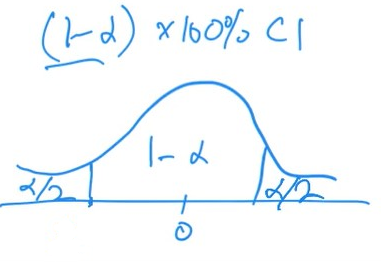
\includegraphics{images/standardnormpdf} 

}

\caption{Standard Normal PDF}\label{fig:stnormpdf}
\end{figure}

Looking at Figure \ref{fig:stnormpdf}, we can see that the section in the middle corresponds to the \(1-\alpha\) percentile, that's our 95\% CI.

The sections on the left and right must be equal to \(\alpha/2\) since for a standard normal pdf, the whole thing must add up to exactly 1.

These two \(\alpha/2\) sections on the left and right of Figure \ref{fig:stnormpdf} refer to the \(Z_{\alpha/2}\) and \(Z_{1-\alpha/2}\) percentiles, respectively.

\textbf{Note}: Due to symmetry, the two \alpha/2 z-scores will be the same magnitude, i.e.~\(-Z_{\alpha/2}=Z_{1-\alpha/2}\). We can use this fact to our advantage.

One could say that the probability we are in the middle area of Figure \ref{fig:stnormpdf} is:

\begin{equation}
P(Z_{\alpha/2}\le Z\le Z_{1-\alpha/2})=1-\alpha
\end{equation}

Equation \eqref{eq:zstannorm} implies that:

\begin{equation}
P(Z_{\alpha/2}\le \frac{\bar{x}-\mu}{\sigma/\sqrt{n}}\le Z_{1-\alpha/2})=1-\alpha
\end{equation}

To isolate \(\mu\) in the above equation, we can substitute \(Z_{\alpha/2}\) with \(-Z_{1-\alpha/2}\) from earlier, then multiply by \(-\sigma/\sqrt{n}\), and finally add \(\bar{x}\) to get:

\begin{equation}
P(\bar{x}+Z_{1-\alpha/2}\frac{\sigma}{\sqrt{n}}\ge \mu \ge \bar{x}-Z_{1-\alpha/2}\frac{\sigma}{\sqrt{n}}) = 1-\alpha
\label{eq:moederived}
\end{equation}

So this means that the population mean must be within the interval given by \(\bar{x}\pm Z_{1-\alpha/2}\frac{\sigma}{\sqrt{n}}\), which is the definition of our confidence interval.

So how do we get the numerical value of the Z-score?

Type qnorm(percentile) in R to find z\_percentile.

So, if \(1-\alpha = 0.95\), then \(1-\alpha/2 = 0.975\), then to R we go\ldots{}

\begin{Shaded}
\begin{Highlighting}[]
\FunctionTok{qnorm}\NormalTok{(}\FloatTok{0.975}\NormalTok{)}
\end{Highlighting}
\end{Shaded}

\begin{verbatim}
## [1] 1.959964
\end{verbatim}

\(\approx 2\)

Voila!

pnorm is the inverse of qnorm:

pnorm(z-score) = percentile qnorm(percentile) = z-score

\subsubsection{Exercise}\label{exercise}

\begin{enumerate}
\def\labelenumi{\arabic{enumi}.}
\tightlist
\item
  Find the z multiplier at 90\% confidence
\end{enumerate}

for 90\% confidence, \(1-\alpha=0.90\), so \(1-\alpha/2=0.95\), so plugging into R

\begin{Shaded}
\begin{Highlighting}[]
\FunctionTok{qnorm}\NormalTok{(}\FloatTok{0.95}\NormalTok{)}
\end{Highlighting}
\end{Shaded}

\begin{verbatim}
## [1] 1.644854
\end{verbatim}

\begin{enumerate}
\def\labelenumi{\arabic{enumi}.}
\setcounter{enumi}{1}
\tightlist
\item
  Find the z multiplier at 98\% confidence
\end{enumerate}

for 98\% confidence \(1-\alpha=0.98\), so \(1-\alpha/2=0.99\)

\begin{Shaded}
\begin{Highlighting}[]
\FunctionTok{qnorm}\NormalTok{(}\FloatTok{0.99}\NormalTok{)}
\end{Highlighting}
\end{Shaded}

\begin{verbatim}
## [1] 2.326348
\end{verbatim}

\begin{enumerate}
\def\labelenumi{\arabic{enumi}.}
\setcounter{enumi}{2}
\tightlist
\item
  Find the z multiplier at 99\% confidence
\end{enumerate}

for 99\% confidence \(1-\alpha=0.99\), so \(1-\alpha/2=0.995\)

\begin{Shaded}
\begin{Highlighting}[]
\FunctionTok{qnorm}\NormalTok{(}\FloatTok{0.995}\NormalTok{)}
\end{Highlighting}
\end{Shaded}

\begin{verbatim}
## [1] 2.575829
\end{verbatim}

\textbf{Question}: Do you notice a trend in the \emph{z} multiplier as confidence level increases? Does this make sense?

\begin{itemize}
\tightlist
\item
  The multiplier increases as the confidence level increases. This makes sense because as the confidence level increases, the range that \(1-\alpha\) encompasses must expand, meaning the \emph{z} multiplier must also increase in kind. In other words, we're more confident our sample mean contains the population mean because we increased our margin of error.
\end{itemize}

Looking back at Equation \eqref{eq:moederived}, is anything strange?

\(\bar{x}\pm Z_{1-\alpha/2}\frac{\sigma}{\sqrt{n}}\)

\(\sigma\) represents population variance, which is rarely known! So how can we apply this formula?

Using sample variance is the right direction.

\begin{center}\rule{0.5\linewidth}{0.5pt}\end{center}

\subsection{t distributions}\label{t-distributions}

Recall that the population variance is

\begin{equation}
\sigma^2 = \frac{\sum{(x_i-\mu)^2}}{N}
\end{equation}

and the sample variance is

\begin{equation}
s^2 = \frac{\sum{(x_i-\bar{x})^2}}{n-1}
\end{equation}

When \(\sigma\) is \textbf{unknown}, we use the sample standard deviation, \emph{s}, to estimate \(\sigma\).

\begin{itemize}
\tightlist
\item
  Previously we computed the standard deviation of sample mean, \(sd(\bar{x})\), as \(\frac{\sigma}{\sqrt{n}}\).
\item
  When \(\sigma\) is unknown, we compute the \textbf{standard error} of the sample mean: \(se(\bar{x})=\frac{s}{\sqrt{n}}\).
\end{itemize}

When the standard deviation of a statistic is estimated from the data, the result is the \textbf{standard error of the statistic}.

In reality, we'll calculate the standard error much more frequently.

\textbf{Scenario}: A random sample of size \emph{n} is drawn from \(N(\mu,\sigma)\).

\begin{itemize}
\tightlist
\item
  When \(\sigma\) is known, \(\bar{x}\approx N(\mu,\frac{\sigma}{\sqrt{n}})\), and so \(Z=\frac{\bar{x}-\mu}{\sigma/\sqrt{n}}\approx N(0,1)\)
\item
  When \(\sigma\) is known and estimated using \emph{s}, the sampling distribution of \(\frac{\bar{x}-\mu}{\sigma/\sqrt{n}}\) is approximated by a \emph{t} \textbf{distribution with degrees of freedom} \emph{n}-1.
\item
  If we do not have a normal proportion, the approximation to the \emph{t} distribution works well if we have a large enough sample size.
\end{itemize}

\subsubsection{Degrees of Freedom}\label{degrees-of-freedom}

\begin{itemize}
\tightlist
\item
  \emph{t} distributions are specified by their \textbf{degrees of freedom}.
\item
  We specify \emph{t} distributions using \emph{t\_k}, where \emph{k} is the degrees of freedom.
\end{itemize}

So CI for \(\mu\), df: \(k=n-1\) since we lose one degree of freedom because the equality \(\frac{\sum{x_i}}{n}=\bar{x}\) must hold.

\subsubsection{\texorpdfstring{\emph{t} Distribution vs Standard Normal}{t Distribution vs Standard Normal}}\label{t-distribution-vs-standard-normal}

Both distributions are centered at 0, symmetric, and bell-shaped. Their differences are: - \emph{t\_k} has associated degrees of freedom. - \emph{t\_k} has slightly \textbf{larger spread}. As the sample size (degrees of freedom) increases, \emph{t\_k} approaches the standard normal.

\emph{t} distribution has more area at extremes or tails of pdf.

\subsubsection{Confidence Interval for Population Mean}\label{confidence-interval-for-population-mean-1}

We use \emph{s} to estimate \(\sigma\) when it is unknown. THe level \emph{C} CI for a population mean becomes:

\begin{equation}
\bar{x}\pm t_{1-\alpha/2,k}\frac{s}{\sqrt{n}}
\label{eq:ciestimate}
\end{equation}

Where \(t_{1-\alpha/2,k}\) is the value from the \emph{t\_k} curve with area \emph{C} between \(t_{\alpha/2,k}\) and \(t_{1-\alpha/2,k}\). The degrees of freedom is \(k=n-1\).

\subsubsection{Finding Multiplier}\label{finding-multiplier}

In R, type qt(percentile, df) to find \emph{t\_\{percentile,df\}}. 1. Find the \emph{t} multiplier at 90\% confidence with 10df

\begin{Shaded}
\begin{Highlighting}[]
\FunctionTok{qt}\NormalTok{(.}\DecValTok{95}\NormalTok{,}\DecValTok{10}\NormalTok{)}
\end{Highlighting}
\end{Shaded}

\begin{verbatim}
## [1] 1.812461
\end{verbatim}

\begin{enumerate}
\def\labelenumi{\arabic{enumi}.}
\setcounter{enumi}{1}
\tightlist
\item
  Find the \emph{t} multiplier at 92\% confidence with 35df
\end{enumerate}

\begin{Shaded}
\begin{Highlighting}[]
\FunctionTok{qt}\NormalTok{(.}\DecValTok{96}\NormalTok{,}\DecValTok{35}\NormalTok{)}
\end{Highlighting}
\end{Shaded}

\begin{verbatim}
## [1] 1.803024
\end{verbatim}

\begin{enumerate}
\def\labelenumi{\arabic{enumi}.}
\setcounter{enumi}{2}
\tightlist
\item
  Find the \emph{t} multiplier at 98\% confidence with 50df
\end{enumerate}

\begin{Shaded}
\begin{Highlighting}[]
\FunctionTok{qt}\NormalTok{(.}\DecValTok{99}\NormalTok{,}\DecValTok{50}\NormalTok{)}
\end{Highlighting}
\end{Shaded}

\begin{verbatim}
## [1] 2.403272
\end{verbatim}

\subsubsection{Worked Example: Banks' Loan-to-Deposit Ratio (LTDR)}\label{worked-example-banks-loan-to-deposit-ratio-ltdr}

\textbf{Question}: The sample mean LTDR for 110 randomly selected American banks is 76.7 and the sample standard deviation is 12.3. Compute a 95\% CI for the population mean LTDR. Based on this CI, is it reasonable to say that the average LTDR is less than 80 for the population?

So, stating our variables:

\begin{Shaded}
\begin{Highlighting}[]
\NormalTok{n}\OtherTok{\textless{}{-}}\DecValTok{110}
\NormalTok{xbar}\OtherTok{\textless{}{-}}\FloatTok{76.7}
\NormalTok{s}\OtherTok{\textless{}{-}}\FloatTok{12.3}
\end{Highlighting}
\end{Shaded}

Using Equation \eqref{eq:ciestimate}:

\begin{equation}
\bar{x}\pm t_{1-\alpha/2,k}\frac{s}{\sqrt{n}}
\end{equation}

and plugging in our variables we get:

\begin{equation}
76.7\pm t_{1-\alpha/2,k}\frac{12.3}{\sqrt{110}}
\end{equation}

and \(t_{1-\alpha/2,k}\) is found using qt(percentile,df), where percentile is \(0.95+\frac{1-0.95}{2} = 0.975\) and \(df=n-1=110-1=109\):

\begin{Shaded}
\begin{Highlighting}[]
\FunctionTok{qt}\NormalTok{(}\FloatTok{0.975}\NormalTok{,}\DecValTok{109}\NormalTok{)}
\end{Highlighting}
\end{Shaded}

\begin{verbatim}
## [1] 1.981967
\end{verbatim}

So plugging this back into Equation \eqref{eq:ciestimate} we get margin of error equal to:

\begin{Shaded}
\begin{Highlighting}[]
\FunctionTok{qt}\NormalTok{(}\FloatTok{0.975}\NormalTok{,n}\DecValTok{{-}1}\NormalTok{)}\SpecialCharTok{*}\NormalTok{s}\SpecialCharTok{/}\FunctionTok{sqrt}\NormalTok{(n)}
\end{Highlighting}
\end{Shaded}

\begin{verbatim}
## [1] 2.32437
\end{verbatim}

So our 95\% CI is given by:

\(76.7\pm 2.3\) or \((74.4,79.0)\)

So, it is reasonable to say that the average LTDR is less than 80 for the population. In other words we're 95\% sure that the average LTDR for the population is less than 80.

Or say:

Yes, since the entire CI is less than 80.

\newpage

\section{Hypothesis Testing}\label{hypothesis-testing}

\subsection{Hypotheses}\label{hypotheses}

\subsubsection{Motivation}\label{motivation-1}

The general approach to hypothesis testing is the following: we perform probability calculations to distinguish patterns seen in data between those that are due to \textbf{chance} and those that \textbf{reflect a real feature} of the phenomenon under study.

\subsubsection{Example}\label{example-1}

You are in charge of quality control in your food company. You randomly sample 40 apcks of cherry tomatoes, each labeled 1/2 lb. (227 g), and find their average weight is 226.5 g. Obviously, we cannot expect boxes filled with whole tomatoes to all weight exactly half a pound. Thus, - is the weight in our sample due to chance? - is the weight in our sample evidence the machine that sorts the tomatoes needs revision?

\subsubsection{Stating Hypotheses}\label{stating-hypotheses}

Hypothesis testing uses sample data to decide on the validity of a hypothesis. A \textbf{hypothesis} is an assumption or a theory about the characteristics of one or more variables in one or more populations. - What you want to know: does the calibrating machine that sorts cherry tomatoes into packs need revision? - The same question reframed statistically: Is the population mean \(\mu\) for the distribution of weights of cherry tomato packages different from 227 g (i.e., half a pound)?

The statement being tested in a test of significance is called the \textbf{null hypothesis}, \(H_0\). The test of significance is designed to assess the strength of the evidence against the null hypothesis. The null hypothesis is usually a statement of ``no effect'' or ``no difference.''

The \textbf{alternative hypothesis}, \(H_a\) is the statement we suspect is true instead of the null hypothesis.

\begin{itemize}
\tightlist
\item
  \(H_0: \mu=227g\)
\item
  \(H_a: \mu\ne227g\)
\end{itemize}

\subsubsection{One-sided and Two-sided Tests}\label{one-sided-and-two-sided-tests}

\begin{itemize}
\item
  A two-sided test of the population mean has the following hypotheses

  \begin{itemize}
  \tightlist
  \item
    \(H_0: \mu=\text{specific number } (\mu_0)\)
  \item
    \(H_a: \mu \ne \text{specific number } (\mu_0)\)
  \end{itemize}
\item
  A one-sided test of the population mean has the following hypotheses

  \begin{itemize}
  \tightlist
  \item
    \(H_0: \mu=\text{specific number } (\mu_0)\)
  \item
    \(H_a: \mu < \text{specific number } (\mu_0)\)
  \end{itemize}

  OR

  \begin{itemize}
  \tightlist
  \item
    \(H_0: \mu = \text{specific number } (\mu_0)\)
  \item
    \(H_a: \mu > \text{specific number } (\mu_0)\)
  \end{itemize}
\end{itemize}

What determines the choice of a one-sided versus a two-sided test is what we know about the problem \textbf{before} we perform a test of statistical significance.

\textbf{Question}: You are in charge of quality control in your food company. You randomly sample 40 apcks of cherry tomatoes, each labeled 1/2 lb. (227 g), and find their average weight is 226.5 g. A consumer advocacy group is trying to claim that consumers are being cheated by the food company. What should the null and alternative hypotheses be in this scenario?

\begin{itemize}
\tightlist
\item
  \(H_0: \mu=227g\)
\item
  \(H_a: \mu<227g\)
\end{itemize}

Consumers would only be cheated if the weight of tomatoes they got was \textbf{less than} the amount on the package.

\begin{center}\rule{0.5\linewidth}{0.5pt}\end{center}

\subsection{Evaluating Evidence: p-values}\label{evaluating-evidence-p-values}

Next, we evaluate the evidence our data provides \textbf{against} the null hypothesis. This evaluation is done by - assuming the null hypothesis is true - computing a test statistic to measure how dissimilar our sample is with the null hypothesis - comparing our test statistic with a benchmark to decide if we have enough evidence against the null hypothesis We then end by making a relevant conclusion

\subsubsection{Test Statistics}\label{test-statistics}

\begin{itemize}
\tightlist
\item
  The test statistic measures how dissimilar our sampled data is with the null hypothesis.
\item
  In a hypothesis test for a mean the test statistic is \begin{equation}
  t=\frac{\bar{x}-\mu_0}{s/\sqrt{n}}
  \label{eq:hyptstmean}
  \end{equation} where \(\mu_0\) represents the value in the null hypothesis \(H_0\)
\item
  The larger (in magnitude) the test statistic, the more evidence we have against the null hypothesis.
\end{itemize}

\subsubsection{Statistic Level}\label{statistic-level}

Before deciding if our test statistic provides enough evidence against the null hypothesis, we first decide on an appropriate \textbf{significance level}, \(\alpha\). THe scientific standard is 0.05, although this value should change based on the context of your problem

\begin{itemize}
\tightlist
\item
  The significance level, \(\alpha\), is the probability of wrongly rejecting the null hypothesis (when the null hypothesis is true, a false positive).
\item
  The benchmark with which we decide if we have enough evidence against the null hypothesis is based on \(\alpha\). There are actually two, equivalent, approaches.
\end{itemize}

\subsubsection{The p-value Approach}\label{the-p-value-approach}

\textbf{p-value}: The probability of obtaining your particular random sample result (or more extreme) if the null hypothesis, \(H_0\), were true.

\begin{itemize}
\tightlist
\item
  A high p-value implies that a random sample result is consistent with \(H_0\).
\item
  A small p-value implies that a random variation alone is unlikely to account for the difference between \(H_0\) and the observation from our random sample. Our sample is inconsistent with \(H_0\).
\item
  The smaller the p-value, the stronger the evidence against \(H_0\).
\item
  With a small p-value we reject \(H_0\), and say that our data support \(H_a\). We reject \(H_0\) when the p-value is \textbf{less than} the significance level, \(\alpha\).
\end{itemize}

\subsubsection{Distribution of a Statistic}\label{distribution-of-a-statistic}

Since the test statistic for testing a mean is Equation \eqref{eq:hyptstmean}, \begin{equation}
t=\frac{\bar{x}-\mu_0}{s/\sqrt{n}} \tag{\@ref{eq:hyptstmean} revisited}
\end{equation} our test statistic is compared with a \emph{t\_k} distribution.

\subsubsection{Finding the p-value}\label{finding-the-p-value}

The p-value is represented by the area under the sampling distribution for values at least as extreme, in the direction of \(H_a\), as that of our random sample.

\begin{itemize}
\tightlist
\item
  In this case, the \emph{sampling distribution} is a \emph{t}-distribution.
\end{itemize}

Assuming the \(H_0\) is true, \(t\approx t_k\) where \(k=n-1\).

\begin{itemize}
\tightlist
\item
  \(H_a: \mu \ne \mu_0\) (two sided test)
\end{itemize}

To find area under distribution for all points greater than the magnitude of \emph{t}, or \(|t|\) in R, use *pt(\(-|t|,df\)) then multiply by two for both tails of the distribution.

\begin{itemize}
\tightlist
\item
  One Sided test

  \begin{itemize}
  \tightlist
  \item
    \(H_a: \mu < \mu_0\), use pt\((t,df)\), since you just want all area to the left of \emph{t}.
  \item
    You are looking for the probability that the population mean is less than the sample mean.
  \item
    \(H_a: \mu > \mu_0\), use \(1-\)pt\((t,df)\), since you want all area to the right of \emph{t}.
  \item
    You are looking for the probability that the population mean is greater than the sample mean.
  \end{itemize}
\end{itemize}

\subsubsection{Decision}\label{decision}

We compare the p-value with the \textbf{significance level}, \(\alpha\).

\begin{itemize}
\tightlist
\item
  If the p-value is less than or equal to \(\alpha\), we reject \(H_0\). Our data support \(H_a\).
\item
  If the p-value is greater than \(\alpha\), we fail to reject \(H_0\). Our data do not support \(H_a\).

  \begin{itemize}
  \tightlist
  \item
    Does not mean we support the null hypothesis, just weren't able to reject it.
  \end{itemize}
\end{itemize}

Rejecting \(H_0\) is said to be a ``statistically significant result''. Failing to reject \(H_0\) is said to be a ``statistically insignificant result''.

\begin{center}\rule{0.5\linewidth}{0.5pt}\end{center}

\subsection{Evaluating Evidence: Critical Value Approach}\label{evaluating-evidence-critical-value-approach}

\textbf{Critical value}: the value of the test statistic that results in a p-value equal to the significance level

\begin{itemize}
\tightlist
\item
  The larger the test statistic, the more evidence we have against \(H_0\).
\item
  If the magnitude of the test statistic is larger than the critical value, we reject \(H_0\).
\end{itemize}

\subsubsection{Finding the Critical Value}\label{finding-the-critical-value}

Critical value, \emph{t}*: the value of t-statistic whose p-value is equal to significance level, \(\alpha\).

\begin{figure}

{\centering 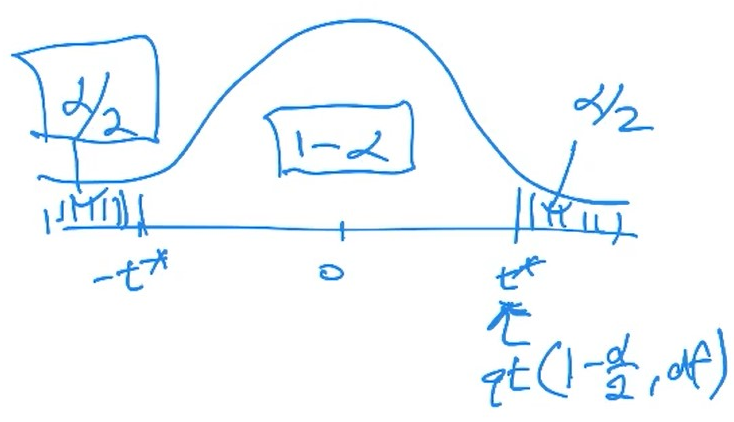
\includegraphics{images/critval2sided} 

}

\caption{t* for 2-Sided Critical Value}\label{fig:2sidecv}
\end{figure}

As seen in Figure \ref{fig:2sidecv}, the value of \emph{t}* for a two-sided test will be given by typing into R the following:

qt(1-\(\frac{\alpha}{2}\),df)

This is because \emph{t}* will be the area in the region \(1-\alpha + \alpha/2 = 1-\alpha/2\)

\textbf{Nota bene}: Remember that qt and pt are the approximations of qnorm and pnorm, respectively, which take into account the degrees of freedom.

For a one sided test, we have two possible scenarios

\begin{itemize}
\item
  \(H_a: \mu > \mu_0\) in this case, the area to the right of \emph{t}* will be represented by \(\alpha\), so we will type qt(1-\(\alpha\)) to find \emph{t}*.
\item
  \(H_a: \mu < \mu_0\) in this case, the area to the left of - \emph{t}* will be represented by \(\alpha\), so we will type qt(\(\alpha\)) to find - \emph{t}*, or -qt(\(\alpha\)) to find \emph{t}*
\end{itemize}

\textbf{Note}: By symmetry notice that -qt(\(\alpha\)) = qt(1-\(\alpha\),df), thus typically for a one-sided test we will typically use qt(1-\(\alpha\),df).

In review:

\begin{itemize}
\tightlist
\item
  Two-sided test

  \begin{itemize}
  \tightlist
  \item
    qt(1-\(\frac{\alpha}{2}\),df)
  \end{itemize}
\item
  One-sided test

  \begin{itemize}
  \tightlist
  \item
    qt(1-\(\alpha\),df)
  \end{itemize}
\end{itemize}

\subsubsection{Exercises}\label{exercises}

\begin{enumerate}
\def\labelenumi{\arabic{enumi}.}
\tightlist
\item
  Find critical value of two-sided \emph{t}-test at \(\alpha=0.1\) with 10 df.
\end{enumerate}

\begin{Shaded}
\begin{Highlighting}[]
\FunctionTok{qt}\NormalTok{(}\DecValTok{1}\FloatTok{{-}0.1}\SpecialCharTok{/}\DecValTok{2}\NormalTok{,}\DecValTok{10}\NormalTok{)}
\end{Highlighting}
\end{Shaded}

\begin{verbatim}
## [1] 1.812461
\end{verbatim}

\begin{enumerate}
\def\labelenumi{\arabic{enumi}.}
\setcounter{enumi}{1}
\tightlist
\item
  Find critical value of one-sided \emph{t}-test at \(\alpha=0.02\) with 55 df.
\end{enumerate}

\begin{Shaded}
\begin{Highlighting}[]
\FunctionTok{qt}\NormalTok{(}\DecValTok{1}\FloatTok{{-}0.02}\NormalTok{,}\DecValTok{55}\NormalTok{)}
\end{Highlighting}
\end{Shaded}

\begin{verbatim}
## [1] 2.103607
\end{verbatim}

\begin{enumerate}
\def\labelenumi{\arabic{enumi}.}
\setcounter{enumi}{2}
\tightlist
\item
  Find critical value of one-sided \emph{t}-test at \(\alpha=0.01\) with 70 df.
\end{enumerate}

\begin{Shaded}
\begin{Highlighting}[]
\FunctionTok{qt}\NormalTok{(}\DecValTok{1}\FloatTok{{-}0.01}\NormalTok{,}\DecValTok{70}\NormalTok{)}
\end{Highlighting}
\end{Shaded}

\begin{verbatim}
## [1] 2.380807
\end{verbatim}

\begin{center}\rule{0.5\linewidth}{0.5pt}\end{center}

\subsection{Summary}\label{summary}

\begin{itemize}
\tightlist
\item
  Based on your question of interest, write \(H_0\) and \(H_a\).
\item
  Evaluate how dissimilar your sample is from \(H_0\) by calculating the test statistic.
\item
  Compare you sample with a benchmark. Two equivalent approaches:

  \begin{enumerate}
  \def\labelenumi{\arabic{enumi}.}
  \tightlist
  \item
    Compare p-value with significance level \(\alpha\).
  \item
    Compare your test statistic with the critical value.
  \end{enumerate}
\item
  Write relevant conclusion for your analysis
\end{itemize}

\begin{center}\rule{0.5\linewidth}{0.5pt}\end{center}

\subsection{Worked Examples}\label{worked-examples}

\textbf{Question 1}: You are in charge of quality control in your food company. You randomly sample 40 packs of cherry tomatoes, each labeled 1/2 lb. (227 g), and find their average weight is 226.5 g. Is the weight in our sample evidence that the machine that sorts the tomatoes needs revision? Suppose the sample standard deviation is 1.5 g.

I think I'd want a two-sided test, so first we find the test statistic using Equation \eqref{eq:hyptstmean},

\(t=\frac{\bar{x}-\mu_0}{s/\sqrt{n}}\),

plug that into pt(t,df), then compare to significance value of 0.05.

So,

\(t=\frac{226.5-227}{1.5/\sqrt{40}}=-2.108\)

\begin{Shaded}
\begin{Highlighting}[]
\FunctionTok{pt}\NormalTok{((}\FloatTok{226.5}\DecValTok{{-}227}\NormalTok{)}\SpecialCharTok{/}\NormalTok{(}\FloatTok{1.5}\SpecialCharTok{/}\FunctionTok{sqrt}\NormalTok{(}\DecValTok{40}\NormalTok{)),}\DecValTok{39}\NormalTok{)}
\end{Highlighting}
\end{Shaded}

\begin{verbatim}
## [1] 0.020746
\end{verbatim}

Multiplying this by 2 (to account for both sides of the distribution) to get our p-value gives us \(\text{p-value}\approx 0.04\).

Since this is less than the significance level of 0.05, we reject the null hypothesis. This is enough evidence that the machine needs revision. Stated statistically, the probability, or p-value, that we would get a sample mean of 226.5 g or less if the true population mean, or \(\mu\), was actually equal to 227 g is so low (\(\approx 4\%\)), that we cannot say this is a chance happening and something is amiss with the sorting machine.

\textbf{Using the Critical Value Method}

\begin{itemize}
\tightlist
\item
  This time we find \emph{t}* using the significance level \(\alpha=0.05\) and compare to the absolute value of our \emph{t-stat} which we previously found to be -2.108.
\item
  use qt(1-alpha/2,df)
\end{itemize}

\begin{Shaded}
\begin{Highlighting}[]
\FunctionTok{qt}\NormalTok{(}\DecValTok{1}\FloatTok{{-}0.05}\SpecialCharTok{/}\DecValTok{2}\NormalTok{,}\DecValTok{39}\NormalTok{)}
\end{Highlighting}
\end{Shaded}

\begin{verbatim}
## [1] 2.022691
\end{verbatim}

Since \(t^*<t\), we reject the null hypothesis. Our data support the claim that the population average weight of cherry tomato packs is different from 227 g.

\textbf{Question 2}: A consumer advocacy group is trying to claim that consumers are being cheated by the food company. Carry out an appropriate hypothesis test.

\begin{itemize}
\tightlist
\item
  \(H_a: \mu > \mu_0\)
\end{itemize}

Only difference here from Question 1 is that now \(t=0.95\) since for a one-sided test \(t=1-\alpha\). So,

\begin{Shaded}
\begin{Highlighting}[]
\FunctionTok{qt}\NormalTok{(}\FloatTok{0.95}\NormalTok{,}\DecValTok{39}\NormalTok{)}
\end{Highlighting}
\end{Shaded}

\begin{verbatim}
## [1] 1.684875
\end{verbatim}

\begin{center}\rule{0.5\linewidth}{0.5pt}\end{center}

\newpage

\section{Practice Questions}\label{practice-questions}

\subsection{Sampling Distributions}\label{sampling-distributions-1}

\begin{enumerate}
\def\labelenumi{\arabic{enumi}.}
\tightlist
\item
  Statistical theory tells us the distribution of the sample means with a fixed sample size, under certain circumstances. The sampling distribution is an approximation of the density histogram of the sample means. WE know the sample means vary from sample to sample. The sampling distribution tells us the expected value (mean) of the distribution, and the standard deviation of the sample means.
\end{enumerate}

\begin{enumerate}
\def\labelenumi{\alph{enumi}.}
\tightlist
\item
  Suppose the variable \emph{X} follows a normal distribution with mean \(\mu\) and standard deviation \(\sigma\). Consider taking random samples, each with size \emph{n}, repeatedly. What is the sampling distribution of the mean?
\end{enumerate}

The sampling distribution is \(N(\mu,\frac{\sigma}{\sqrt{n}})\) since \(X\approx N(\mu,\sigma)\)

\begin{enumerate}
\def\labelenumi{\alph{enumi}.}
\setcounter{enumi}{1}
\tightlist
\item
  Suppose the variable \emph{X} has an unknown distribution but known mean \(\mu\) and known standard deviation \(\sigma\). What is the name of the statistical theory that informs us that the sampling distribution of the sample mean, \(\bar{x}\), can be well-approximated by a normal distribution?
\end{enumerate}

The Central Limit Theorem

\begin{enumerate}
\def\labelenumi{\arabic{enumi}.}
\setcounter{enumi}{1}
\tightlist
\item
  An automatic machine in a manufacturing process produces sub-components. The lengths of the sub-components follow a normal distribution of the sample mean of 116 cm and a standard deviation of 4.8 cm.
\end{enumerate}

\begin{enumerate}
\def\labelenumi{\alph{enumi}.}
\tightlist
\item
  Find the probability that one selected sub-component is longer than 118 cm.
\end{enumerate}

Z-score here is \(\frac{118-116}{4.8}\)

\begin{Shaded}
\begin{Highlighting}[]
\DecValTok{1}\SpecialCharTok{{-}}\FunctionTok{pnorm}\NormalTok{(}\DecValTok{2}\SpecialCharTok{/}\FloatTok{4.8}\NormalTok{)}
\end{Highlighting}
\end{Shaded}

\begin{verbatim}
## [1] 0.3384611
\end{verbatim}

\begin{enumerate}
\def\labelenumi{\alph{enumi}.}
\setcounter{enumi}{1}
\tightlist
\item
  Find the probability that if 3 sub-components are randomly selected, their mean length exceeds 118 cm.
\end{enumerate}

z-score here is \(\frac{118-116}{4.8/\sqrt{3}}\)

\begin{Shaded}
\begin{Highlighting}[]
\NormalTok{zscore}\OtherTok{\textless{}{-}}\NormalTok{(}\DecValTok{118{-}116}\NormalTok{)}\SpecialCharTok{/}\NormalTok{(}\FloatTok{4.8}\SpecialCharTok{/}\FunctionTok{sqrt}\NormalTok{(}\DecValTok{3}\NormalTok{))}
\DecValTok{1}\SpecialCharTok{{-}}\FunctionTok{pnorm}\NormalTok{(zscore)}
\end{Highlighting}
\end{Shaded}

\begin{verbatim}
## [1] 0.2352432
\end{verbatim}

\subsection{Confidence Intervals}\label{confidence-intervals-1}

\begin{enumerate}
\def\labelenumi{\arabic{enumi}.}
\setcounter{enumi}{2}
\tightlist
\item
  What are the goals of constructing a confidence interval?
\end{enumerate}

\begin{itemize}
\tightlist
\item
  A confidence interval shows in what range we expect to find a sample mean (range of plausible values)
\item
  provide estimate for unknown parameter of interest
\item
  provide measure of uncertainty
\end{itemize}

\begin{enumerate}
\def\labelenumi{\arabic{enumi}.}
\setcounter{enumi}{3}
\tightlist
\item
  How does increasing the confidence level affect the margin of error and the width of the confidence interval? Hint: sketching the standard normal distribution will be helpful
\end{enumerate}

\begin{itemize}
\tightlist
\item
  When the confidence level increases, the margin of error and the width of the confidence interval increase as well. This is because we can be more certain the unknown parameter is contained within the confidence interval when it is wider, but this also increases the range within which it can be found, leading to a larger margin of error.
\end{itemize}

\begin{enumerate}
\def\labelenumi{\arabic{enumi}.}
\setcounter{enumi}{4}
\tightlist
\item
  How does increasing the sample size affect the margin of error and width of the confidence interval? Briefly explain.
\end{enumerate}

\begin{itemize}
\tightlist
\item
  Increasing the sample size decreases the margin of error and width of confidence interval. This is because the margin of error and width of confidence interval are proportional to \(\frac{1}{\sqrt{n}}\) where \emph{n} is the sample size. So increasing \emph{n} decreases the MOE and CI width.
\end{itemize}

\begin{enumerate}
\def\labelenumi{\arabic{enumi}.}
\setcounter{enumi}{5}
\tightlist
\item
  Use R to find the value of the t-multiplier when constructing a confidence interval for the mean in the following situations:
\end{enumerate}

\begin{enumerate}
\def\labelenumi{(\alph{enumi})}
\tightlist
\item
  94\% CI with \(n=49\).
\end{enumerate}

\begin{Shaded}
\begin{Highlighting}[]
\FunctionTok{qt}\NormalTok{(.}\DecValTok{97}\NormalTok{,}\DecValTok{48}\NormalTok{)}
\end{Highlighting}
\end{Shaded}

\begin{verbatim}
## [1] 1.926298
\end{verbatim}

\begin{enumerate}
\def\labelenumi{(\alph{enumi})}
\setcounter{enumi}{1}
\tightlist
\item
  86\% CI with \(n=82\).
\end{enumerate}

\begin{Shaded}
\begin{Highlighting}[]
\FunctionTok{qt}\NormalTok{(.}\DecValTok{93}\NormalTok{,}\DecValTok{81}\NormalTok{)}
\end{Highlighting}
\end{Shaded}

\begin{verbatim}
## [1] 1.490412
\end{verbatim}

\begin{enumerate}
\def\labelenumi{(\alph{enumi})}
\tightlist
\item
  74\% CI with \(n=150\).
\end{enumerate}

\begin{Shaded}
\begin{Highlighting}[]
\FunctionTok{qt}\NormalTok{(.}\DecValTok{87}\NormalTok{,}\DecValTok{149}\NormalTok{)}
\end{Highlighting}
\end{Shaded}

\begin{verbatim}
## [1] 1.130695
\end{verbatim}

\begin{enumerate}
\def\labelenumi{\arabic{enumi}.}
\setcounter{enumi}{6}
\tightlist
\item
  A random sample of 100 students had a mean grade point average (GPA) of 3.2 with a standard deviation of 0.2.
\end{enumerate}

\begin{enumerate}
\def\labelenumi{\alph{enumi}.}
\tightlist
\item
  Calculate a 97\% CI for the mean GPA for all students
\end{enumerate}

\begin{itemize}
\item
  Confidence interval is given by \(\bar{x} \pm t_{mult} \times \frac{s}{\sqrt{n}}\)
\item
  Where the right half is the MOE. So,
\end{itemize}

\begin{Shaded}
\begin{Highlighting}[]
\FunctionTok{qt}\NormalTok{(}\FloatTok{0.985}\NormalTok{,}\DecValTok{99}\NormalTok{)}\SpecialCharTok{*}\FloatTok{0.2}\SpecialCharTok{/}\FunctionTok{sqrt}\NormalTok{(}\DecValTok{100}\NormalTok{)}
\end{Highlighting}
\end{Shaded}

\begin{verbatim}
## [1] 0.04403637
\end{verbatim}

\begin{itemize}
\tightlist
\item
  So confidence interval is \(3.2 \pm 0.044\) or (3.156,3.244)
\end{itemize}

\begin{enumerate}
\def\labelenumi{\alph{enumi}.}
\setcounter{enumi}{1}
\tightlist
\item
  What is the margin of error for the confidence interval found in the previous part? what is the margin of error telling us?
\end{enumerate}

\begin{itemize}
\tightlist
\item
  The margin of error is about 0.044 grade points. This tells us the range within which we expect the true mean GPA to be; it also gives us a measure of uncertainty of the mean GPA.
\end{itemize}

\begin{enumerate}
\def\labelenumi{\alph{enumi}.}
\setcounter{enumi}{2}
\tightlist
\item
  Based on this confidence interval, is it reasonable to say that the mean GPA of all students is 3.25 or greater?
\end{enumerate}

\begin{itemize}
\tightlist
\item
  Because 3.25 falls outside of our confidence interval, it is unlikely that that the true mean GPA of all students is 3.25 or greater.
\end{itemize}

\subsection{Hypothesis Testing}\label{hypothesis-testing-1}

\begin{enumerate}
\def\labelenumi{\arabic{enumi}.}
\setcounter{enumi}{7}
\tightlist
\item
  What is the goal of conducting a hypothesis test?
\end{enumerate}

\begin{itemize}
\tightlist
\item
  The goal of hypothesis testing is to determine the likelihood of obtaining a particular sample mean
\item
  distinguish if sample statistic is due to random chance or reflects a real feature of phenomenon under study
\end{itemize}

\begin{enumerate}
\def\labelenumi{\arabic{enumi}.}
\setcounter{enumi}{8}
\tightlist
\item
  Hypothesis statements are always about the \textbf{population / sample statistic} (choose one) of interest.
\end{enumerate}

\begin{itemize}
\tightlist
\item
  sample statistic
\end{itemize}

\begin{enumerate}
\def\labelenumi{\arabic{enumi}.}
\setcounter{enumi}{9}
\tightlist
\item
  For each of the situations, state the appropriate null and alternative hypotheses, in symbols and in words. Sketch how you would find the p-value based on the calculated test-statistic.
\end{enumerate}

\begin{enumerate}
\def\labelenumi{\alph{enumi}.}
\tightlist
\item
  David's car averages 29 miles per gallon on the highway. He just switched to a new motor oil that is advertised as increasing gas mileage. He wants to investigate if the advertisement is accurate.
\end{enumerate}

\begin{itemize}
\tightlist
\item
  \(H_0: \mu = 29 \text{ mpg}\)
\item
  \(H_a: \mu < 29 \text{ mpg}\)
\end{itemize}

\begin{enumerate}
\def\labelenumi{\alph{enumi}.}
\setcounter{enumi}{1}
\tightlist
\item
  The diameter of a spindle in a small motor is supposed to be 4 millimeters. If the spindle is too small or too large, the motor will not function properly. The manufacturer wants to investigate further whether the mean diameter is moved away from the target.
\end{enumerate}

\begin{itemize}
\tightlist
\item
  \(H_0: \mu = 4 \text{ mm}\)
\item
  \(H_a: \mu \ne 4 \text{ mm}\)
\end{itemize}

\begin{enumerate}
\def\labelenumi{\alph{enumi}.}
\setcounter{enumi}{2}
\tightlist
\item
  The average time in traffic between 2 points of a congested highway used to be 2 hours. The government invested money to improve travel times by building extra lanes and overpasses. Citizens want to access if travel times have improved, on average.
\end{enumerate}

\begin{itemize}
\tightlist
\item
  \(H_0: \mu = 2 \text{ hr}\)
\item
  \(H_a: \mu < 2 \text{ hr}\)
\end{itemize}

\begin{enumerate}
\def\labelenumi{\arabic{enumi}.}
\setcounter{enumi}{10}
\tightlist
\item
  To have more evidence against the null hypothesis, our test statistic should be \textbf{larger / smaller} (choose one) in magnitude. Briefly explain.
\end{enumerate}

\begin{itemize}
\tightlist
\item
  Larger, since the test statistic is a measure of how dissimilar the sampled data is from the null hypothesis, a larger test statistic is more evidence against the null hypothesis.
\end{itemize}

\begin{enumerate}
\def\labelenumi{\arabic{enumi}.}
\setcounter{enumi}{11}
\tightlist
\item
  How does increasing the difference between the sample mean and the population mean under the null hypothesis affect the test statistic and the evidence against the null hypothesis?
\end{enumerate}

\begin{itemize}
\tightlist
\item
  Increasing the difference between the sample mean and population mean will increase the test statistic and provide more evidence against the null hypothesis.
\end{itemize}

\begin{enumerate}
\def\labelenumi{\arabic{enumi}.}
\setcounter{enumi}{12}
\tightlist
\item
  How does increasing the sample size affect the test statistic and the evidence against the null hypothesis?
\end{enumerate}

\begin{itemize}
\tightlist
\item
  Test statistic is given by \(t=\frac{\bar{x}-\mu}{s/\sqrt{n}}=\frac{(\bar{x}-\mu)\sqrt{n}}{s}\), so an increase in sample size will also increase the test-statistic and provide more evidence against the null hypothesis.
\end{itemize}

\begin{enumerate}
\def\labelenumi{\arabic{enumi}.}
\setcounter{enumi}{13}
\tightlist
\item
  Use R to obtain the critical values of the following hypothesis tests:
\end{enumerate}

-find t-stat whose p-value is equal to the significance level \(\alpha\).

\begin{enumerate}
\def\labelenumi{\alph{enumi}.}
\tightlist
\item
  \(H_0: \mu = 3.5, H_a: \mu \ne 3.5, \text{ with } \alpha=0.8 \text{ and } n=96\)
\end{enumerate}

\begin{Shaded}
\begin{Highlighting}[]
\FunctionTok{qt}\NormalTok{(}\FloatTok{0.96}\NormalTok{,}\DecValTok{95}\NormalTok{)}
\end{Highlighting}
\end{Shaded}

\begin{verbatim}
## [1] 1.769615
\end{verbatim}

\begin{enumerate}
\def\labelenumi{\alph{enumi}.}
\setcounter{enumi}{1}
\tightlist
\item
  \(H_0: \mu = 75, H_a: \mu < 75, \text{ with } \alpha=0.12 \text{ and } n=43\)
\end{enumerate}

\begin{Shaded}
\begin{Highlighting}[]
\FunctionTok{qt}\NormalTok{(}\FloatTok{0.88}\NormalTok{,}\DecValTok{42}\NormalTok{)}
\end{Highlighting}
\end{Shaded}

\begin{verbatim}
## [1] 1.191879
\end{verbatim}

\begin{enumerate}
\def\labelenumi{\alph{enumi}.}
\setcounter{enumi}{2}
\tightlist
\item
  \(H_0: \mu = 10, H_a: \mu > 10, \text{ with } \alpha=0.045 \text{ and } n=132\)
\end{enumerate}

\begin{Shaded}
\begin{Highlighting}[]
\FunctionTok{qt}\NormalTok{(}\DecValTok{1}\FloatTok{{-}0.045}\NormalTok{,}\DecValTok{131}\NormalTok{)}
\end{Highlighting}
\end{Shaded}

\begin{verbatim}
## [1] 1.708027
\end{verbatim}

\begin{enumerate}
\def\labelenumi{\arabic{enumi}.}
\setcounter{enumi}{14}
\tightlist
\item
  Use R to obtain the p-values of the following hypothesis tests:
\end{enumerate}

\begin{enumerate}
\def\labelenumi{\alph{enumi}.}
\tightlist
\item
  \(H_0: \mu=48, H_a: \mu \ne 48, \text{ with } t-stat=2.14 \text{ and } n=50.\)
\end{enumerate}

\begin{itemize}
\tightlist
\item
  for a two sided test, multiply p-value by 2 to account for both sides
\end{itemize}

\begin{Shaded}
\begin{Highlighting}[]
\NormalTok{(}\DecValTok{1}\SpecialCharTok{{-}}\FunctionTok{pt}\NormalTok{(}\FloatTok{2.14}\NormalTok{,}\DecValTok{49}\NormalTok{))}\SpecialCharTok{*}\DecValTok{2}
\end{Highlighting}
\end{Shaded}

\begin{verbatim}
## [1] 0.03735955
\end{verbatim}

\begin{enumerate}
\def\labelenumi{\alph{enumi}.}
\setcounter{enumi}{1}
\tightlist
\item
  \(H_0: \mu=3, H_a: \mu >3, \text{ with } t-stat=0.78 \text{ and } n=316.\)
\end{enumerate}

\begin{Shaded}
\begin{Highlighting}[]
\DecValTok{1}\SpecialCharTok{{-}}\FunctionTok{pt}\NormalTok{(}\FloatTok{0.78}\NormalTok{,}\DecValTok{315}\NormalTok{)}
\end{Highlighting}
\end{Shaded}

\begin{verbatim}
## [1] 0.2179883
\end{verbatim}

\begin{enumerate}
\def\labelenumi{\alph{enumi}.}
\setcounter{enumi}{2}
\tightlist
\item
  \(H_0: \mu=12, H_a: \mu <12, \text{ with } t-stat=1.57 \text{ and } n=34.\)
\end{enumerate}

\begin{Shaded}
\begin{Highlighting}[]
\FunctionTok{pt}\NormalTok{(}\FloatTok{1.57}\NormalTok{,}\DecValTok{33}\NormalTok{)}
\end{Highlighting}
\end{Shaded}

\begin{verbatim}
## [1] 0.9370224
\end{verbatim}

\begin{enumerate}
\def\labelenumi{\arabic{enumi}.}
\setcounter{enumi}{15}
\tightlist
\item
  The 10-year historical average yield of corn in the United States is 160 bushels per acre. A survey of 50 farmers this year gives a sample mean yield of 158.4 bushels per acre, with a standard deviation of 5 bushels per acre. Does this sample provide evidence that the yield of corn has decreased from the 10-year historical average? Conduct an appropriate hypothesis test.
\end{enumerate}

\begin{enumerate}
\def\labelenumi{\alph{enumi}.}
\tightlist
\item
  State the null and alternative hypotheses.
\end{enumerate}

\begin{itemize}
\tightlist
\item
  \(H_0: \mu = 160 \text{ bushels per acre}\)
\item
  \(H_a: \mu < 160 \text{ bushels per acre}\)
\end{itemize}

\begin{enumerate}
\def\labelenumi{\alph{enumi}.}
\setcounter{enumi}{1}
\tightlist
\item
  Calculate the test-statistic.
\end{enumerate}

\begin{itemize}
\tightlist
\item
  Given by \(t^* = \frac{\bar{x}-\mu}{s/\sqrt{n}}\) so,
\end{itemize}

\begin{Shaded}
\begin{Highlighting}[]
\NormalTok{tstar16}\OtherTok{\textless{}{-}}\NormalTok{(}\FloatTok{158.4}\DecValTok{{-}160}\NormalTok{)}\SpecialCharTok{/}\NormalTok{((}\DecValTok{5}\SpecialCharTok{/}\FunctionTok{sqrt}\NormalTok{(}\DecValTok{50}\NormalTok{)))}
\NormalTok{tstar16}
\end{Highlighting}
\end{Shaded}

\begin{verbatim}
## [1] -2.262742
\end{verbatim}

\begin{enumerate}
\def\labelenumi{\alph{enumi}.}
\setcounter{enumi}{2}
\tightlist
\item
  Find the p-value and the critical value.
\end{enumerate}

\begin{itemize}
\tightlist
\item
  Usign significance level, \(\alpha\), of 0.05:
\item
  \textbf{p-value approach}
\end{itemize}

\begin{Shaded}
\begin{Highlighting}[]
\FunctionTok{pt}\NormalTok{(tstar16,}\DecValTok{49}\NormalTok{)}
\end{Highlighting}
\end{Shaded}

\begin{verbatim}
## [1] 0.01405941
\end{verbatim}

\begin{itemize}
\tightlist
\item
  \textbf{critical value approach}
\end{itemize}

\begin{Shaded}
\begin{Highlighting}[]
\FunctionTok{qt}\NormalTok{(}\FloatTok{0.95}\NormalTok{,}\DecValTok{49}\NormalTok{)}
\end{Highlighting}
\end{Shaded}

\begin{verbatim}
## [1] 1.676551
\end{verbatim}

\begin{enumerate}
\def\labelenumi{\alph{enumi}.}
\setcounter{enumi}{3}
\tightlist
\item
  State a conclusion in context.
\end{enumerate}

\begin{itemize}
\tightlist
\item
  Because the p-value is less than the significance level, and because the critical value is less than the magnitude of the t-statistic, we must reject the null hypothesis. Our data support the claim that the yield of corn this year has decreased from the 10-year historical average.
\end{itemize}

\begin{enumerate}
\def\labelenumi{\alph{enumi}.}
\setcounter{enumi}{4}
\tightlist
\item
  How would you interpret the calculated p-value?
\end{enumerate}

\begin{itemize}
\tightlist
\item
  There is a probability of 0.014 that we will obtain a sample mean of 158.4 bushels per acre if the average yield this year is truly 160 bushels per acre.
\end{itemize}

\subsection{General Questions}\label{general-questions}

\begin{enumerate}
\def\labelenumi{\arabic{enumi}.}
\setcounter{enumi}{16}
\tightlist
\item
  Obtain the critical value of a hypothesis test where \(H_0: \mu=145,H_a: \mu \ne 145,\text{ with significance level } \alpha=0.02\). Suppose the sample size is 50.
\end{enumerate}

\begin{itemize}
\tightlist
\item
  This is a \textbf{two-sided} test, so I'll use qt(\(1-\alpha/2\),df)
\end{itemize}

\begin{Shaded}
\begin{Highlighting}[]
\FunctionTok{qt}\NormalTok{(}\FloatTok{0.99}\NormalTok{,}\DecValTok{49}\NormalTok{)}
\end{Highlighting}
\end{Shaded}

\begin{verbatim}
## [1] 2.404892
\end{verbatim}

\begin{enumerate}
\def\labelenumi{\arabic{enumi}.}
\setcounter{enumi}{17}
\tightlist
\item
  Obtain the t-multiplier for a 98\% confidence interval. Suppose the sample size is 50.
\end{enumerate}

\begin{itemize}
\tightlist
\item
  To find t-multiplier, I'll use qt(\(1-\alpha/2\),df)
\end{itemize}

\begin{Shaded}
\begin{Highlighting}[]
\FunctionTok{qt}\NormalTok{(}\FloatTok{0.99}\NormalTok{,}\DecValTok{49}\NormalTok{)}
\end{Highlighting}
\end{Shaded}

\begin{verbatim}
## [1] 2.404892
\end{verbatim}

\begin{enumerate}
\def\labelenumi{\arabic{enumi}.}
\setcounter{enumi}{18}
\tightlist
\item
  Compare the critical value and the t-multiplier found in the previous two parts. What is the implication based on this comparison?
\end{enumerate}

\begin{itemize}
\tightlist
\item
  The two values are equal. The implication is that conclusions from a two-sided hypothesis test conducted at significance level \(\alpha\) will be consistent with conclusions from a \((1-\alpha) \times\) 100\% confidence interval.
\end{itemize}

\begin{enumerate}
\def\labelenumi{\arabic{enumi}.}
\setcounter{enumi}{19}
\tightlist
\item
  Suppose the hypothesis test in question 17 is carried out and the p-value is 0.043. Which of the following confidence intervals is/are possible?
\end{enumerate}

\begin{itemize}
\item
  (143.2,144.5)
\item
  (151.3,154.6)
\item
  (144.5,163.5)
\item
  Since the p-value is higher than the significance level, \(\alpha=0.02\), we fail to reject the null hypothesis. Thus 145 must fall within the confidence interval, so only the CI (144.5,163.5) is possible.
\end{itemize}

\begin{enumerate}
\def\labelenumi{\arabic{enumi}.}
\setcounter{enumi}{20}
\tightlist
\item
  A random sample of 85 banded archerfish were collected, and their lengths were measured and recorded. Their average length was 20cm with a standard deviation of 3cm.
\end{enumerate}

\begin{enumerate}
\def\labelenumi{\alph{enumi}.}
\tightlist
\item
  Construct a 95\% confidence interval for the population mean length of banded archerfish.
\end{enumerate}

\begin{itemize}
\tightlist
\item
  So \(\alpha = 0.05\) since the CI is 95\%. Need to find t-multiplier and variance \(\frac{s}{\sqrt{n}}\)
\end{itemize}

\begin{Shaded}
\begin{Highlighting}[]
\FunctionTok{qt}\NormalTok{(}\FloatTok{0.975}\NormalTok{,}\DecValTok{84}\NormalTok{)}\SpecialCharTok{*}\DecValTok{3}\SpecialCharTok{/}\FunctionTok{sqrt}\NormalTok{(}\DecValTok{85}\NormalTok{)}
\end{Highlighting}
\end{Shaded}

\begin{verbatim}
## [1] 0.647085
\end{verbatim}

\begin{itemize}
\tightlist
\item
  CI is \(20\pm 0.647\) or (19.353,20.647)
\end{itemize}

\begin{enumerate}
\def\labelenumi{\alph{enumi}.}
\setcounter{enumi}{1}
\tightlist
\item
  Based on your confidence interval, is it plausible that the population mean length of banded archerfish is 21cm? Briefly explain.
\end{enumerate}

\begin{itemize}
\tightlist
\item
  It is not plausible that the population mean length is 21cm since 21cm falls outside of the 95\% confidence interval.
\end{itemize}

\begin{enumerate}
\def\labelenumi{\alph{enumi}.}
\setcounter{enumi}{2}
\tightlist
\item
  Suppose you conduct the following hypothesis test. \(H_0: \mu=21,H_a:\mu \ne 21\). Without actually performing any additional calculations, what do you expect the p-value of this hypothesis test will be? Briefly explain.
\end{enumerate}

\begin{itemize}
\item
  greater than 0.05
\item
  less than 0.05
\item
  The p-value will be smaller than 0.05, since this means that if the the probability that a sample mean will be 21.
\end{itemize}

\begin{enumerate}
\def\labelenumi{\alph{enumi}.}
\setcounter{enumi}{3}
\tightlist
\item
  Conduct the hypothesis test to verify your answer to the previous part.
\end{enumerate}

\begin{itemize}
\tightlist
\item
  Find p-value using pt()
\end{itemize}

\begin{Shaded}
\begin{Highlighting}[]
\NormalTok{t21}\OtherTok{\textless{}{-}}\NormalTok{(}\DecValTok{20{-}21}\NormalTok{)}\SpecialCharTok{/}\NormalTok{(}\DecValTok{3}\SpecialCharTok{/}\FunctionTok{sqrt}\NormalTok{(}\DecValTok{85}\NormalTok{))}
\NormalTok{t21}
\end{Highlighting}
\end{Shaded}

\begin{verbatim}
## [1] -3.073181
\end{verbatim}

\begin{Shaded}
\begin{Highlighting}[]
\DecValTok{2}\SpecialCharTok{*}\FunctionTok{pt}\NormalTok{(t21,}\DecValTok{84}\NormalTok{)}
\end{Highlighting}
\end{Shaded}

\begin{verbatim}
## [1] 0.002855487
\end{verbatim}

\begin{itemize}
\tightlist
\item
  Find critical value
\end{itemize}

\begin{Shaded}
\begin{Highlighting}[]
\FunctionTok{qt}\NormalTok{(}\FloatTok{0.975}\NormalTok{,}\DecValTok{84}\NormalTok{)}
\end{Highlighting}
\end{Shaded}

\begin{verbatim}
## [1] 1.98861
\end{verbatim}

\begin{itemize}
\tightlist
\item
  Since this is lower than \(\alpha=0.05\) and the magnitude of the critical value (1.989 \textless{} \textbar-3.073\textbar) we reject the null hypothesis. Our data supports the claim that the population mean does not equal 21cm.
\end{itemize}

\chapter{Basics of R}\label{basics-of-r}

\section{Getting Started with R}\label{getting-started-with-r}

\subsection{Question 1}\label{question-1}

\textbf{(a)}

\begin{Shaded}
\begin{Highlighting}[]
\NormalTok{cars.df}\OtherTok{\textless{}{-}}\NormalTok{mtcars}
\end{Highlighting}
\end{Shaded}

\textbf{(b)}
According to the environment window, there are 32 observations of 11 variables in the dataset \emph{mtcars}.

\subsection{Question 2}\label{question-2}

\textbf{(a)}

\begin{Shaded}
\begin{Highlighting}[]
\NormalTok{students.df}\OtherTok{\textless{}{-}}\FunctionTok{read.table}\NormalTok{(}\StringTok{"datasets/students.txt"}\NormalTok{,}\AttributeTok{header=}\ConstantTok{TRUE}\NormalTok{)}
\end{Highlighting}
\end{Shaded}

\textbf{(b)}
According to the environment window, there are 249 observations of 9 variables in the dataset \emph{students.txt}.

\subsection{Question 3}\label{question-3}

\textbf{(a) - (h)}

The packages \emph{tidyverse, faraway, MASS, leaps, ROCR, nycflights13, gapminder, palmerpenguins} were installed.

\subsection{Question 4}\label{question-4}

\begin{Shaded}
\begin{Highlighting}[]
\FunctionTok{library}\NormalTok{(faraway)}
\NormalTok{corn.df}\OtherTok{\textless{}{-}}\NormalTok{cornnit}
\end{Highlighting}
\end{Shaded}

\section{Topic B.3: Data Types \& Structures in R}\label{topic-b.3-data-types-structures-in-r}

\subsection{Question 5}\label{question-5}

\textbf{(a)} 2020\_Major Valid

\textbf{(b)} .2020.Age Invalid, number follows .

\textbf{(c)} \#Courses.2020 Invalid, \# not allowed

\textbf{(d)} \_courses\_2020 Invalid, cannot start with underscore

\textbf{(e)} Fav\_Sport20 Valid

\textbf{(f)} major 2020 Invalid, space not allowed

\textbf{(g)} age(2020) Invalid, parentheses not allowed

\textbf{(h)} FavSport\_2020 Valid

\subsection{Question 6}\label{question-6}

\begin{Shaded}
\begin{Highlighting}[]
\NormalTok{practice}\OtherTok{\textless{}{-}}\FunctionTok{c}\NormalTok{(}\DecValTok{13}\NormalTok{,}\DecValTok{91}\NormalTok{,}\DecValTok{36}\NormalTok{,}\DecValTok{95}\NormalTok{,}\DecValTok{9}\NormalTok{,}\DecValTok{3}\NormalTok{,}\DecValTok{61}\NormalTok{,}\DecValTok{20}\NormalTok{,}\DecValTok{22}\NormalTok{,}\DecValTok{97}\NormalTok{)}
\FunctionTok{class}\NormalTok{(practice)}
\end{Highlighting}
\end{Shaded}

\begin{verbatim}
## [1] "numeric"
\end{verbatim}

\subsection{Question 7}\label{question-7}

\textbf{(a)} practice{[}5{]}==5 False

\begin{Shaded}
\begin{Highlighting}[]
\NormalTok{practice[}\DecValTok{5}\NormalTok{]}\SpecialCharTok{==}\DecValTok{5}
\end{Highlighting}
\end{Shaded}

\begin{verbatim}
## [1] FALSE
\end{verbatim}

\textbf{(b)} practice{[}10{]}!=97 False

\begin{Shaded}
\begin{Highlighting}[]
\NormalTok{practice[}\DecValTok{10}\NormalTok{]}\SpecialCharTok{!=}\DecValTok{97} 
\end{Highlighting}
\end{Shaded}

\begin{verbatim}
## [1] FALSE
\end{verbatim}

\textbf{(c)} (practice{[}1{]}+practice{[}2{]})\textless104 False

\begin{Shaded}
\begin{Highlighting}[]
\NormalTok{(practice[}\DecValTok{1}\NormalTok{]}\SpecialCharTok{+}\NormalTok{practice[}\DecValTok{2}\NormalTok{])}\SpecialCharTok{\textless{}}\DecValTok{104}
\end{Highlighting}
\end{Shaded}

\begin{verbatim}
## [1] FALSE
\end{verbatim}

\textbf{(d)} (practice{[}1{]}+practice{[}2{]})\textless=104 True

\begin{Shaded}
\begin{Highlighting}[]
\NormalTok{(practice[}\DecValTok{1}\NormalTok{]}\SpecialCharTok{+}\NormalTok{practice[}\DecValTok{2}\NormalTok{])}\SpecialCharTok{\textless{}=}\DecValTok{104}
\end{Highlighting}
\end{Shaded}

\begin{verbatim}
## [1] TRUE
\end{verbatim}

\textbf{(e)} (practice{[}2{]}==91) \& (practice{[}9{]}==22) True * True=True

\begin{Shaded}
\begin{Highlighting}[]
\NormalTok{(practice[}\DecValTok{2}\NormalTok{]}\SpecialCharTok{==}\DecValTok{91}\NormalTok{) }\SpecialCharTok{\&}\NormalTok{ (practice[}\DecValTok{9}\NormalTok{]}\SpecialCharTok{==}\DecValTok{22}\NormalTok{)}
\end{Highlighting}
\end{Shaded}

\begin{verbatim}
## [1] TRUE
\end{verbatim}

\textbf{(f)} (practice{[}5{]}\textless9) \textbar{} (practice{[}6{]}\textgreater=4) False + False = False

\begin{Shaded}
\begin{Highlighting}[]
\NormalTok{(practice[}\DecValTok{5}\NormalTok{]}\SpecialCharTok{\textless{}}\DecValTok{9}\NormalTok{) }\SpecialCharTok{|}\NormalTok{ (practice[}\DecValTok{6}\NormalTok{]}\SpecialCharTok{\textgreater{}=}\DecValTok{4}\NormalTok{)}
\end{Highlighting}
\end{Shaded}

\begin{verbatim}
## [1] FALSE
\end{verbatim}

\subsection{Question 8}\label{question-8}

\begin{Shaded}
\begin{Highlighting}[]
\NormalTok{Mat.A}\OtherTok{\textless{}{-}}\FunctionTok{matrix}\NormalTok{(}\FunctionTok{c}\NormalTok{(}\DecValTok{4}\NormalTok{,}\DecValTok{6}\NormalTok{,}\DecValTok{1}\NormalTok{,}\DecValTok{2}\NormalTok{,}\DecValTok{3}\NormalTok{,}\DecValTok{1}\NormalTok{),}\AttributeTok{nrow =} \DecValTok{2}\NormalTok{,}\AttributeTok{ncol =} \DecValTok{3}\NormalTok{)}

\NormalTok{Mat.A}
\end{Highlighting}
\end{Shaded}

\begin{verbatim}
##      [,1] [,2] [,3]
## [1,]    4    1    3
## [2,]    6    2    1
\end{verbatim}

\textbf{(a)}

\begin{Shaded}
\begin{Highlighting}[]
\FunctionTok{colnames}\NormalTok{(Mat.A)}\OtherTok{\textless{}{-}}\FunctionTok{c}\NormalTok{(}\StringTok{"Huey"}\NormalTok{,}\StringTok{"Dewey"}\NormalTok{,}\StringTok{"Louie"}\NormalTok{)}

\NormalTok{Mat.A}
\end{Highlighting}
\end{Shaded}

\begin{verbatim}
##      Huey Dewey Louie
## [1,]    4     1     3
## [2,]    6     2     1
\end{verbatim}

\textbf{(b)} Output of Mat.A{[}2,1{]} would be 6.

\begin{Shaded}
\begin{Highlighting}[]
\NormalTok{Mat.A[}\DecValTok{2}\NormalTok{,}\DecValTok{1}\NormalTok{]}
\end{Highlighting}
\end{Shaded}

\begin{verbatim}
## Huey 
##    6
\end{verbatim}

\textbf{(c)} Output of dim(Mat.A) would be (2,3).

\begin{Shaded}
\begin{Highlighting}[]
\FunctionTok{dim}\NormalTok{(Mat.A)}
\end{Highlighting}
\end{Shaded}

\begin{verbatim}
## [1] 2 3
\end{verbatim}

\subsection{Question 9}\label{question-9}

\begin{Shaded}
\begin{Highlighting}[]
\FunctionTok{factor}\NormalTok{(practice)}
\end{Highlighting}
\end{Shaded}

\begin{verbatim}
##  [1] 13 91 36 95 9  3  61 20 22 97
## Levels: 3 9 13 20 22 36 61 91 95 97
\end{verbatim}

The order of the levels in the factor \emph{practice} are:
3 9 13 20 22 36 61 91 95 97

\section{R Markdown}\label{r-markdown}

\subsection{Question 10}\label{question-10}

As evidenced by the above, my answers were typed up using R Markdown, and an HTML file was created.

  \bibliography{book.bib,packages.bib}

\end{document}
